% EE Thesis/Dissertation
% Please see http://ee.tamu.edu/~tex for information about EE Thesis.

%==================================================
%This is the Special Study Document
%==================================================

\documentclass[12pt,a4paper]{aitthesis}
%\documentclass[12pt,a4paper]{article}

\usepackage{graphicx}
\usepackage{latexsym}
\usepackage{amssymb,amsthm,amsmath}
%\usepackage[notocbib]{apacite}
\usepackage{apacite}
\usepackage{verbatim}
\usepackage{multirow}
\usepackage{bm}
%\usepackage{url}
\usepackage{algorithm}
\usepackage{algcompatible}
\usepackage{placeins}
\usepackage{times}
\usepackage{array}
\usepackage[caption=false,font=footnotesize]{subfig}
\usepackage{pdflscape}

\usepackage[hyphenbreaks]{breakurl}
\usepackage[hyphens]{url}
\usepackage{tabulary}
\usepackage[utf8]{inputenc}
\usepackage{longtable}
\usepackage{seqsplit}
\usepackage{epigraph}
\usepackage{dirtytalk}
\usepackage[export]{adjustbox}
\usepackage{enumitem}
\usepackage[usenames, dvipsnames]{color}
\usepackage[table]{xcolor}

\newcommand{\oops}[1]{\bf{#1}}
\newcommand{\ga}{\bar{\gamma}}
\newcommand{\myint}{\int_0^{\infty}}
\renewcommand{\vec}[1]{\mathbf{#1}}
\newcommand{\mat}[1]{\mathrm{#1}}

\newcommand{\vectornorm}[1]{\left|\left|#1\right|\right|}

\newcommand{\ten}[1]{\mathcal{#1}}
\newcommand{\crossmat}[1]{\begin{bmatrix} #1 \end{bmatrix}_{\times}}
\newcommand{\class}[1]{{\cal C}_{#1}}
\def\Rset{\mathbb{R}}
\def\Pset{\mathbb{P}}
\DeclareMathOperator*{\argmax}{argmax}
\DeclareMathOperator*{\argmin}{argmin}
\DeclareMathOperator*{\sign}{sign}
\def\norm{\mbox{$\cal{N}$}}

\newcommand\parms{\vec{\lambda}}
\newcommand\oldparms{\parms^{\text{old}}}


%\def\short{1}

\begin{document}

\pagenumbering{roman}
\pagestyle{plain}
%==========================================================
%======================  FRONT STUFF ======================
%==========================================================

%======================= Cover Page =======================
%\begin{document}
\newpage
\pagestyle{plain}
\pagenumbering{roman}
\setcounter{page}{1}
\addcontentsline{toc}{section}{Title Page}
%\setlength{\footskip}{-15mm}
\setlength{\textheight}{230mm}
\setlength{\voffset}{10mm}
\vskip -5em

\begin{center}
{ 
  \singlespace \uppercase{\bf Comprehensive study of methods techniques and tools used for Data Analytics in fields of Finance } \par
}
\vskip 2em
{
  \lineskip 1.5em
  \begin{tabular}[t]{c} by\\ \\ Parth Sarangi
  \end{tabular}\par
}
%\vskip 5.6em

\vskip 3.5em
\singlespace A special study report submitted in partial fulfillment of the
requirements for the \\ degree of Master of Engineering in\\ 
Information Management

%	\vskip 5em
\vskip 0.5em
{
  \singlespace
  \begin{center}
    \begin{tabular}{rl}
      \\[-1em]
      Examination Committee: & Dr. Vatcharaporn Esichaikul (Chairperson) \\[-0.8em]
                             & Dr. Matthew N. Dailey \\[-0.8em]
                             & Prof. Sumanta Guha \\
\\
% UNCOMMENT THE LINES BELOW IF YOU HAVE THE EXTERNAL EXAMINER.
%      External Examiner:     & Prof.\ YOUR EXTERNAL EXAMINER \\[-0.8em]
%                             & Dept.\ of Electrical and Computer Engineering \\[-0.8em]
%                             & McGill University, Canada \\\\
		
      Nationality:     & Indian \\[-0.8em]
      Previous Degree: & Bachelor of Technology in Electronics and Communication\\[-0.8em]
                       & National Institute of Technology Srinagar, India\\[-0.8em]
      \\
      Scholarship Donor: & AIT Fellowship\\[-0.8em]
      \\
    \end{tabular}
  \end{center}

  \vskip 3.0em
  \centerline{}
  \vskip 2em
}
\end{center}
\begin{center}
  \singlespace Asian Institute of Technology\\ School of Engineering
                  and Technology\\ Thailand\\ April 2017
\end{center}
\vfill
\begin{comment}

-------------------To be uncommented when writing final thesis

%====================== ACKNOWLEDGEMENTS ======================
\newpage
\pagestyle{plain}
\addcontentsline{toc}{section}{Acknowledgments}
\onecolumn % Single-column.
\if@twoside\else\raggedbottom\fi % Ragged bottom unless twoside option.
\setlength{\footskip}{8mm}
\begin{center}
{
  \large \bf Acknowledgments\\ \vskip 1em
}
\vskip 1em
\end{center}
\singlespace
\doublespace
\hspace{8.5mm}
\vspace{-1em}

I would like to thank all my family members for showing great support towards my dream of pursuing a Master’s degree. 
I also thank my Professors Dr. Vatcharaporn Esichaikul and Dr Matthew N. Dailey for guiding me in my academics and for helping me understand the concepts. 
\\
\\
Lastly I also humbly thank the staff of my Institution for their support and assistance in my  academic pursuit.
Above all I am grateful to the ominipresent spirit of the universe which guides me in achieving the milestones I imagined.


%====================== ABSTRACT ======================
\newpage
\pagestyle{plain}
\addcontentsline{toc}{section}{Abstract}
\onecolumn % Single-column.
\if@twoside\else\raggedbottom\fi % Ragged bottom unless twoside option.

\setlength{\footskip}{8mm}

\begin{center}
{\large \bf Abstract \\ \vskip 1em}
\vskip 1em
\end{center}
\singlespace
\doublespace
\hspace{8.5mm}
\vspace{-1em}

The telecom industry is very competitive. There is a huge customer base and they number of players are less. Hence occasional offers from competition results in loss of customer and a drop in revenue. The phenomenon is termed churning and it may occur in any service  industry. 
\\Thus this thesis is to control churning by modeling a system which is capable of identifying the customers. It also proposes decisions which could be taken to retain these customers.

\end{comment}
\setlength{\parskip}{0pt} 




%======================= Table of Contents =========================
\newpage
\addcontentsline{toc}{section}{Table of Contents}
\tableofcontents

% Page 2 begins

%===================== List of Figures ======================
\newpage
\addcontentsline{toc}{section}{List of Figures}
\listoffigures

%\clearpage     % \clearpage ends the page, and also dumps out all floats.
%\end{document} % Floats are things like tables and figures.

%\clearpage     % \clearpage ends the page, and also dumps out all floats.

% %===================== List of Tables ======================
\newpage
\addcontentsline{toc}{section}{List of Tables}
\listoftables

% %\clearpage     % \clearpage ends the page, and also dumps out all floats.
% %\end{document} % Floats are things like tables and figures.

%\clearpage     % \clearpage ends the page, and also dumps out all floats.

\setlength{\parskip}{12pt}


\small

\pagenumbering{arabic}
\setlength{\headheight}{12pt}
\setlength\parskip{\baselineskip}

\pagestyle{plain}

\setlength{\footskip}{8mm}

\chapter{Introduction}


\section{Overview}

Data analysis is an very robust topic in the field of data science and encompasses the various mathematical functions. The functions are statistical in nature and are performed on the data obtained. The goal of data analytics is to support (or reject) the hypothesis which the data scientist postulates.
“ By processing a steady stream of real-time data, organizations can make time-sensitive decisions faster than ever before, monitor emerging trends, course-correct rapidly and jump on new business opportunities.” [BIG Data Analytics: A Framework for Unstructured Data Analysis pdf]

This paper tries to enlist most of the up-to-date techniques used by researchers and mathematicians to make sense of the data. Also the paper presents them in three groups of analytics.
But then there arises a question which is, why the need for data analytics ? Well, to answer that the paper proposes the literature from an article of Kdnuggets \shortcite{KDnuggets}.

According to Paul following are use cases  of data analytics :
1. Analytics powers our decisions – we do not need to guess while making bold new decisions, we should use the information from data at hand.
2. Your data analysis weighs down your opponent's argument.
3. Cut down on loss making ventures with data analytics.
4. Can be applied to all domains be it health-care, banking, marketing, sales, operations etc.
On the scenario when describing Data analytics it is very important to put the focus on Hypothesis.

Shown in the table \ref{tableDMusecase} is some business areas 


\begin{table}[H]
	\centering
%	\hskip-1.8cm
	\begin{tabular}{|p{4cm}|p{4cm}|l|}
		\hline
		\textbf{Application area} & \textbf{Applications} & \textbf{Specifics}\\
		\hline
		Insurance & Fraud detection & Identify claims meriting investigation\\
		\hline
		Telecom & Churn & Identify likely customer turnover\\
		\hline
		Telemarketing & On-line information & Aid telemarketers with easy data access\\
		\hline
		Human resource management & Churn & Identify potential employee turnover\\
		\hline
		\multirow{2}{4em}{Retail}  & Affinity positioning & Position product effectively\\
		& Cross-selling & Find more products for customers\\
		\hline
		\multirow{2}{4em}{Banking} & Customer relationship management & Identify customer value\\
		&& Develop programs to maximize revenue\\
		\hline
		Credit card management & Lift & Identify effective market segments\\
		& Churn & Identify likely customer turnover\\
		\hline
	\end{tabular}
	\caption{Data mining use cases}
	\label{tableDMusecase}
\end{table}
	
Figure \ref{fig:data-analytics} is a view of the data analytics with respect to the main fields.

\begin{figure}[H]
	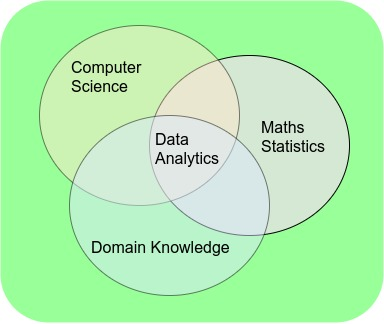
\includegraphics[scale = 0.8]{figures/FlowChart.jpg}
	\centering
	\caption{Data Analytics}
	\label{fig:data-analytics}
\end{figure}

\subparagraph{Why Analytics for financial institutions ?}
Customers are loyal consumers of products, which give value for their monetary investments. Big institutions tend to over look the need for value creation and focus their analytics and metrics to improve profit \shortcite{Reichheld1996}. In the HBR report Reichheld makes certain  observations that customers of large companies witness degrading value standards and secondly increasing rate of customer churn is a good variable to predict cash flow from consumer to company. He also noted that companies can replace old customer with new ones but the profits are lower as cost of induction is high.



	

2. Categories in data analytics :

There are three basic categories viz. Descriptive, Predictive and Prescriptive. The methods and techniques are described further in the paper, and they are classified into the above.

2.1 Descriptive Analytic techniques: The sole purpose of using the methods in this category would be to describe the Hypothesis. Descriptive analytics or data mining are at the bottom of the big data value chain, but they can be valuable for uncovering patterns that offer insight. A simple example of descriptive analytics would be assessing credit risk; using past financial performance to predict a customer’s likely financial performance. Descriptive analytics can be useful in the sales cycle, for example, to categorize customers by their likely product preferences and sales cycle.

To summarize data into meaningful charts and reports, for example, about budgets, sales, revenues, or cost. They allow managers to obtain standard and customized reports, and drill down into the data and to make queries to understand the impact of an advertising campaign, for example, review business performance to find problems or areas of opportunity, and identify patterns and trends in data. Typical questions that descriptive analytics help answer are: How much did we sell in each region? What was our revenue and profit last quarter? How many and what types of complaints did we resolve? Which factory has the lowest productivity? Descriptive analytics also help companies to classify customers into different segments, which enable them to develop specific marketing campaigns and advertising strategies. [1]

There are two main approaches to apply in this topic Data warehousing and Visual analytics with reporting.

2.2 Predictive analytic techniques : Predictive analytics use big data to identify past patterns to predict the future. For example, some companies are using predictive analytics for sales lead scoring. Some companies have gone one step further use predictive analytics for the entire sales process, analyzing lead source, number of communications, types of communications, social media, documents, CRM data, etc. Properly tuned predictive analytics can be used to support sales, marketing, or for other types of complex forecasts.


2.3 Prescriptive analytic techniques : Prescriptive analytics is really valuable, but largely not used. According to Gartner, 13 percent of organizations are using predictive but only 3 percent are using prescriptive analytics. Where big data analytics in general sheds light on a subject, prescriptive analytics gives you a laser-like focus to answer specific questions. For example, in the healthcare industry, you can better manage the patient population by using prescriptive analytics to measure the number of patients who are clinically obese, then add filters for factors like diabetes and LDL cholesterol levels to determine where to focus treatment. The same prescriptive model can be applied to almost any industry target group or problem.


There is yet another classification of Analytics tools on the basis of the generation ie. Traditional vs Advanced.[1] [1 - https://rapidminer.com/summarizing-differences-business-intelligence-advanced-analytics/]

Traditional analytics employ visualizations like graphs, charts (pie, bar), infographics etc., querying, reporting, scorecards and OLAP. They tend to answer the Descriptive analytics type of questions. Generally used in Business Intelligence softwares, just query from existing data and display intuitive infographics, the user deciphers the data. The process of the business intelligence is generally termed as reactive.
Tools in consumer market WebFOCUS InfoAssist OLAP, IBM Cognos, Netweaver, Microstrategy Intelligence Server, andara Balanced Scorecard, BSC designer and any SQL relational database like Oracle, Microsoft Sql Server.
1. OLAP
2.Dashboards
3. Scorecards
4. KPI’s

Advanced analytics, on the other hand go beyond the traditional techniques. They use modeling, optimization, statistics methods to discover the future and predict an outcome. The softwares may also be termed as decision support systems or expert systems as they generate possible deductions. User could use the help and substantiate their own judgments. The process in this category is termed as proactive.
Methods used in advanced analytics are: predictive modeling, Statistical analysis, Simulation and Optimization, Text mining, Data mining, Multimedia mining, Descriptive modeling.
Tools in the consumer market are Powerpivot, Tableau, Qliksense, Yellowfin, etc.
1. Statistical Methods
2. Text Mining
3. Data Mining
4. Multimedia mining
5. Simulation
6. Optimization


3. Fields and Domains of application :



\section{Objectives}

The overall objective of the study report is to understand the major methods, techniques and tools adopted by financial institutions to perform data analytics.



%\section{Thesis Outline}

%The organization of this dissertation is as follows:
%\begin{itemize}
%	\item In Chapter \ref{ch:literature-review}, the literature review is explored.
%	\item In Chapter \ref{ch:methodology}, the methodology is proposed.
%\end{itemize}

%In Chapter \ref{ch:results}, I present the experimental results.
%Finally, in Chapter \ref{ch:conclusion}, I conclude my thesis.

\FloatBarrier

\setlength{\footskip}{8mm}

\chapter{Analytics in financial institutions}

\section{Rationale for use of analytics?}
According to a joint research study, by Boston Consulting Group and Morgan Stanley with analytics professionals, it was reveled that the financial institutions lagged behind other verticals in the use of data analytics~\shortcite{BCGanalytics2017} and it is shown in figure~\ref{fig:da_digitization}. One of the findings of the research was that FI's are investing a lot of capital, an estimated total of about \textdollar1bn. In addition it was found that for near term value creation the FI's expected data analytics to optimize customer acquisition, customer retention, operational efficiency, and risk mitigation.
\newline
\newline
\begin{figure}[H]
	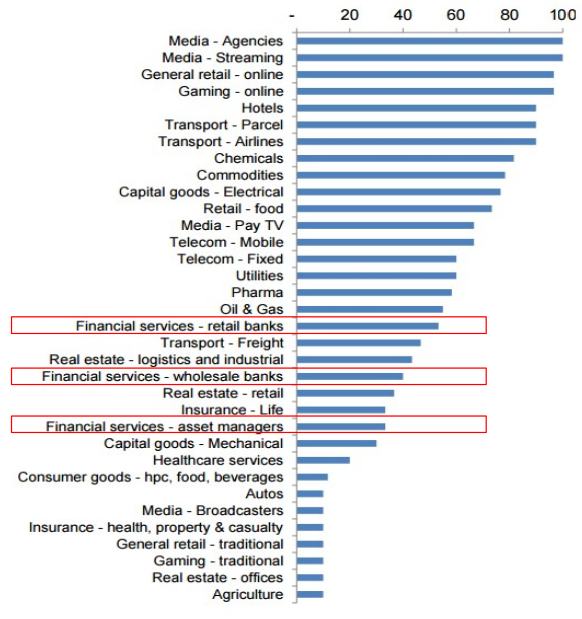
\includegraphics[width=13cm, height=12cm]{figures/DA_used_verticals.png}
	\caption{Reprinted from the Morgan Stanley Digitization Index ranks }
	\label{fig:da_digitization}
\end{figure}
\FloatBarrier

\newpage
\section{State of analytics in financial companies}
From the survey of FI's, a mix of interviewees representing payment companies, service providers, insurance, commercial banks, BCG made some interesting discoveries. It was found that most organizations have invested in analytics techniques to generate market perceptions. Some of the most used were those of social media, log, text and location analytics as shown in figure~\ref{fig:da_capabilities}.

\begin{figure}[H]
	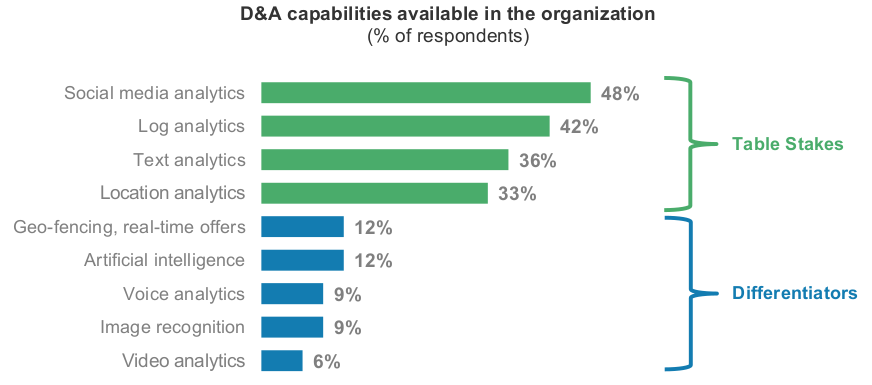
\includegraphics[scale = 0.5]{figures/DA_capabilities.png}
	\caption[Da capablities]{Reprinted from the work of Boston consulting group  }
	\label{fig:da_capabilities}
\end{figure}
\FloatBarrier

Researchers have highlighted that most of the interviewees claimed that institutions are yet to make substantial gain from investments in analytics. They identified that companies can make gains from automation and digitization of manual processes. Additionally, it was noted that financial institutions are adopting digital processes to automate data collection for KYC (Know Your Customer) service and Anti-money laundering 
%\newline
%\newline
Customers are loyal consumers of products, which give value for their monetary investments. Big institutions tend to over look the need for value creation and focus their analytics and metrics to improve profit \shortcite{Reichheld1996}. In the HBR report Reichheld makes certain  observations that customers of large companies witness degrading value standards and secondly increasing rate of customer churn is a good variable to predict cash flow from consumer to company. He also noted that companies can replace old customer with new ones but the profits are lower as cost of induction is high.

\newpage
\section{Challenges faced by analytics}
For every new technology there are certain common challenges, such as those of acceptability and usability. Finding out the actual benefit or Return on investment for newer technologies and solutions such as those of digital assistants remains a mystery. There is no quantifiable or tangible benefit, but only a perception that it could revolutionize the method of banking and investing.
Some hurdles, such as of vision, budget, and getting all members on board, are faced early in the life-cycle of adopting such bold complex projects. Institution leadership faces the tough task of decision making and if rests on them to perceive value at the end of project.
Even after adopting analytics and tools, management faces challenges of educating shareholders, staff and customers to be literate enough to invest and interact with solutions for effective usage.

\section{Types of data mining}
There are broadly defined three categories of analytic techniques, as follows :
\begin{enumerate}
	\item Descriptive analytics elaborated in the chapter~\ref{descriptive-techniques}
	\item Predictive analytics is described in the chapter~\ref{predictive-techniques}
	\item Prescriptive analytics discussed in the chapter~\ref{prescriptive-techniques}
\end{enumerate}

According to Paul following are use cases  of data analytics :
\begin{enumerate}
	\item Analytics powers our decisions – we do not need to guess while making bold new decisions, we should use the information from data at hand.
	\item Your data analysis weighs down your opponent's argument.
	\item Cut down on loss making ventures with data analytics.
	\item Can be applied to all domains be it health-care, banking, marketing, sales, operations etc.
\end{enumerate}

On the scenario when describing Data analytics it is very important to put the focus on Hypothesis.

Shown in the table~\ref{tableDMusecase} is some business areas 


\begin{table}[H]
	\centering
	%	\hskip-1.8cm
	\begin{tabular}{|p{4cm}|p{4cm}|l|}
		\hline
		\textbf{Application area} & \textbf{Applications} & \textbf{Specifics}\\
		\hline
		Insurance & Fraud detection & Identify claims meriting investigation\\
		\hline
		Telecom & Churn & Identify likely customer turnover\\
		\hline
		Telemarketing & On-line information & Aid telemarketers with easy data access\\
		\hline
		Human resource management & Churn & Identify potential employee turnover\\
		\hline
		\multirow{2}{4em}{Retail}  & Affinity positioning & Position product effectively\\
		& Cross-selling & Find more products for customers\\
		\hline
		\multirow{2}{4em}{Banking} & Customer relationship management & Identify customer value\\
		&& Develop programs to maximize revenue\\
		\hline
		Credit card management & Lift & Identify effective market segments\\
		& Churn & Identify likely customer turnover\\
		\hline
	\end{tabular}
	\caption{Data mining use cases}
	\label{tableDMusecase}
\end{table}

Figure \ref{fig:data-analytics} is a view of the data analytics with respect to the main fields.

\begin{figure}[H]
	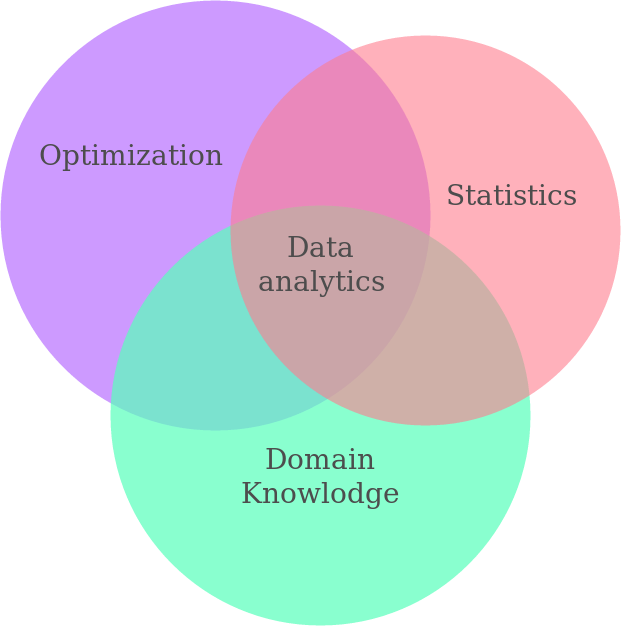
\includegraphics[scale = 0.6]{figures/AnalyticsDomain.png}
	\centering
	\caption{Data Analytics}
	\label{fig:data-analytics}
\end{figure}
\FloatBarrier

Below we see a representations for the advanced analytics and business analytics~\ref{fig:rapidminer-aa}.

\begin{figure}[H]
	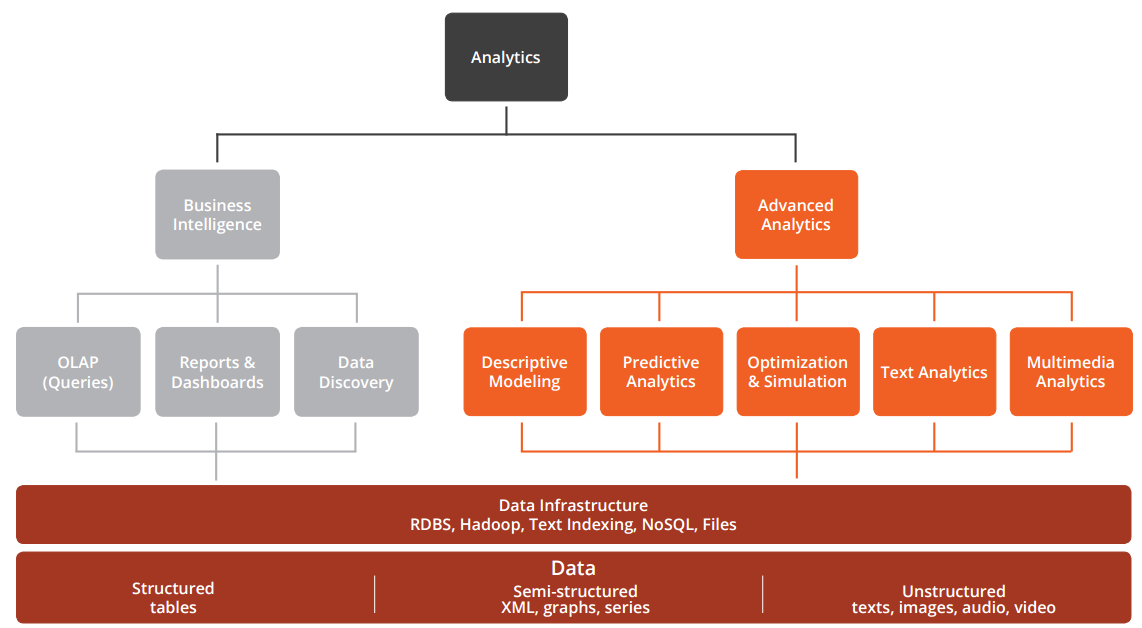
\includegraphics[scale=0.4]{figures/RapidMiner_AdvancedAnalytics_new.png}
	\caption{Advanced analytics}
	\label{fig:rapidminer-aa}
\end{figure}




\chapter{Descriptive Techniques} 
\label{descriptive-techniques}

The sole purpose of using the methods in this category would be to describe the Hypothesis. Descriptive analytics or data mining are at the bottom of the big data value chain, but they can be valuable for uncovering patterns that offer insight. A simple example of descriptive analytics would be assessing credit risk; using past financial performance to predict a customer’s likely financial performance. Descriptive analytics can be useful in the sales cycle, for example, to categorize customers by their likely product preferences and sales cycle.

To summarize data into meaningful charts and reports, for example, about budgets, sales, revenues, or cost. They allow managers to obtain standard and customized reports, and drill down into the data and to make queries to understand the impact of an advertising campaign, for example, review business performance to find problems or areas of opportunity, and identify patterns and trends in data. Typical questions that descriptive analytics help answer are: How much did we sell in each region? What was our revenue and profit last quarter? How many and what types of complaints did we resolve? Which factory has the lowest productivity? Descriptive analytics also help companies to classify customers into different segments, which enable them to develop specific marketing campaigns and advertising strategies.
There are two main approaches to apply in this topic Data warehousing and Visual analytics with reporting.

Descriptive analytics is very common and basic form of data mining technique to derive meaning and trend from data. Almost all of the companies in financial sector utilize the tools based on these techniques. The techniques in this are relatively basic compared with those of predictive models and prescriptive models. Institutions generally use tools which can generate reports regularly, some are printed monthly while some others are generated  as a yearly routine. Such demands for reports describe the status quo of the balance sheets, organizational debts and cash flows. Daly transactions and updates of balances are maintained in the books or accounts and reports are generated daily for accountants and auditors. Thus it is imperative that vital functions of reporting, updating and auditing are functionalities of some business analytics.

There are several techniques employed by businesses to analyze and display data. They are as follows:
\begin{enumerate}
	\item OLAP
	\item Datawarehouse
	\item Graphical views
	\item Performance dashboard and KPI's
	\item Social media analysis
	\item Text analysis
\end{enumerate}

\section{Social media analytics}
In a paper titled ``Social media big data and capital markets—An overview``~\shortcite{bukovina2016social}, the researchers have studied the behavior of relationship between social media and the capital markets. The study relates to as behavioral finance. 

\section{Text analytics}
In a paper titled ``When machines read the news``~\shortcite{gross2011machines}, the authors have used text mining to derive the relation between scrip news and intra-day stock trading. They try to relate the stock price fluctuations and liquidity, to the unscheduled news flash. The researchers used Reuter`s NewScope is an news engine which classifies stock/company related news into positive, negative and neutral segments. The techniques used was VAR model known as vector autoregressive model. This model is used for multivariate time series. 

The data was sourced from Reuter`s NewsScope sentiment engine. It contains around 29,500 records of news headlines in the period of 1 year from the month of July 2007 to June 2008. Each news item has 3 attributes of sentiment, relevance and novelty. 40 stocks listed on the London stock exchange were selected for analysis. These are actively traded on the exchange and thus a dynamic market sentiment and frequent news coverage. These stocks cover about 70\% of the FTSE100 market capitalization. 
According to the data analysis it was found that high frequency trading activity reacts positively to company specific news marked as relevant.

\section{Location analytics}
Valuation of goods and products varies from place to place. A certain item could be priced higher in a remote location compared to a normative value when sold in urban store.
Location analytics is suitable for such marketers to price products according to demand and location. Improper valuation may decrease demand and eventually lead to unprofitable business. For example a bottle of water could cost 10 bucks in a city store, but could be priced about 5 times as high in an airport terminal. 
A research study published in the journal ``Procedia Economics and Finance``, describes the real estate valuations in Romania~\shortcite{droj2015usage}. It compares the evaluation of  studies the economic effects of using Location analytics and the standard practice of 
The study incorporates the use of Cadaster system for spatial analysis in the domain of GIS - Geographical information system. Cadaster system is a technique of mapping 
The researchers used a decision support system integrated with GIS functionality. It can improves manual valuations by taking in financial analysis of the property and fusing with the physical and social environmental influences.
Normal pricing evaluations of properties are based on Hedonic models, ie. they price the individual elements of the properties and add them up. The pricing of bedrooms, kitchen, stories, size, are summed up.
Factors taken into valuation of real estate are as follows :
\begin{itemize}
	\item Physical location 
	\item Social effects of proximity to schools, commercial spots, hospitals, nurseries, parks, criminality, recreational centers.
	\item Infrastructure of neighborhood such as roads, public transportation facilities, water and sewage systems, communications networks and Internet facilities.
	\item Environmental factors of air pollution, noise, industrial pollution, aircraft noise, traffic congestion etc.
	\item Economic price trends
	\item Legal constraints of building or modifying structures
\end{itemize}
In this study, researcher could automate the valuation of properties and determine the precise value. The cadaster system database is continuously updated by the administration with up to date taxation details. Hence it was possible to generate accurate valuations of living spaces.

%
%
%
%

\setlength{\footskip}{8mm}

\chapter{Predictive Techniques} 
\label{predictive-techniques}

The basis of Predictive modeling is the use of data mining techniques to forecast future results. Data mining is the process of sorting data to find patterns or infer relationships. Thus a formulation of a statistical model with relevant variables is essential for prediction~\shortcite{dataMining}. 

Predictive analytics use big data to identify past patterns to predict the future. For example, some companies are using predictive analytics for sales lead scoring. Some companies have gone one step further use predictive analytics for the entire sales process, analyzing lead source, number of communications, types of communications, social media, documents, CRM data, etc. Properly tuned predictive analytics can be used to support sales, marketing, or for other types of complex forecasts~\shortcite{predictiveModelling}.

Data mining techniques are used in credit card systems to detect fraud, in loan approval systems, identifying customer types and targeting specific promotional schemes. It is used to model customer behavior and detect churning to certain financial products. Insurance schemes and bank deposits are volatile instruments due to the uncertainty of the free economy~\shortcite{hbrCustomerdefection}.


%There are many techniques to modeling predictive analytics 
%
%
%\begin{enumerate}
%	\item Clustering methods
%	\item Regession methods
%	\item Classification methods
%	\item Association rules
%\end{enumerate}

%
%
%
%
\newpage
\section{Geo fencing}
Geo-fencing (or also known as Location Analytics) is the term for creating a location based analytics algorithm which can track customers in a certain area and deliver valuable marketing or services. The technology works based on geographic location services and tracks any potential clients with their mobile gps. 
Geo fencing tools are software applications which reside on the 

Use-cases for geofencing :
\begin{itemize}
	\item Manage a group of cargo vehicles
	\item Detect and optimize harbor docking for port management of ships
	\item Density flow of vehicles and management on roads or air space near airports.
	\item Exhibition centers can manage the flow of attendees to optimally view all exhibits, ensuring all items on display can be viewed.
	\item Shopping malls and shops can monitor the passage of people and optimize the display of commercials or products.
\end{itemize}

Geo fences are designed into the application which generally store the latitude and longitudes of the location to be monitored. When the user uses the app, it reads data from the gps module and keeps checking if the client has crossed any geo fence en-route. Now-a-days geo fencing.

Google maps geo fencing is available via API's 

\newpage
\section{Artificial intelligence}
AI was developed a long time ago, but it has for recent years gained much traction and entered our lives. AI was present from the 1950's, but it has only gained popularity.
According to an article by PwC~\shortcite{PwcAI2017}, some companies have invested in AI, Machine and Cognitive learning tools and have implemented solutions for Chatbots, Personal assistants etc. Big data coupled with faster computing and ubiquitous implementation with cloud computing has certainly boosted research and development.
As per a Forbes research projection, in the next 10 years, implementations of AI will increase economic growth by 100\% in about 20 countries. Also there could be an increase in productivity of around 40\% of banks financial labor~\shortcite{Forbes2017}.

AI is used as a technique to automate various categories of tasks such as following~\shortcite{rich1991artificial} :
\begin{itemize}
	\item Mundane tasks
		\begin{itemize}
			\item Perception via Vision and Speech
			\item Natural language processing 
			\item Robot control and common sense
		\end{itemize}
	\item Formal tasks
	\begin{itemize}
		\item Playing games such as chess, go, checkers etc
		\item Solving mathematical problems of geometry, logic, calculus
	\end{itemize}
	\item Expert tasks
	\begin{itemize}
		\item Engineering design, fault finding, Manufacturing planning
		\item Scientific analysis
		\item Medical diagnosis
		\item Financial analysis
	\end{itemize}
\end{itemize}

Some techniques which fall in the space of AI are Support vector machines, Heuristics, Neural networks, Markhov decision process, and NLP natural language processing.

In an example case presented by a researcher from Romania~\shortcite{Costea2014}, the techniques of artificial intelligence combined with fuzzy logic for classification.
The case is applied to a scenario where the National Bank of Romania classifies NFI`s into ``good`` or ``poor`` depending on the periodic financial reporting. The Non - Banking financial institutions of Romania are regulated by governmental policy to send their financial reports to the NBR for scrutiny. NBR appoints their staff to manually screen the reports and classify for goodness or badness and then need to proceed for on site inspection.
The artificial neural network is built with genetic algorithm and trained to perform classification. The process involved introducing mutations to chromosomes of both the parents and offspring.

The dataset is made of 990 records having 11 attributes grouped into 3 dimensions viz., Capital adequacy, assets` quality and profitability. The data ranged between 2007 to 2012. There were 68 non banking financial institutions. 4 clusters were chosen using the Fuzzy C Means algorithm. The ANN structure contained 8 neurons on the first hidden layer and 5 on the next. The accuracy rate achieved was around 92.32\% and validation accuracy around 91\% and testing accuracy about 89\%. Thus in this study the researcher was able to get high accuracy artificial neural network classification to classify the financial statements of non- banking institutions in Romania.


\section{Deep learning}
In the paper ref~\shortcite{heaton2016deep} the authors have presented a list of techniques which are being used to classify and predict financial domain problems ranging from :
\begin{itemize}
	\item securities pricing
	\item portfolio design and entity selection
	\item risk management
\end{itemize}.

Deep learning models are being used in financial product design by working with big data. These models produce better results than the traditional techniques of economics. 

\section{Supervised learning - Decision tree}
The article titled ``What drives gold returns? A decision tree analysis`` ~\shortcite{malliaris2015drives} the authors discuss gold price fluctuations 


%\section{Image recognition}



%\section{Video analytics}



\setlength{\footskip}{8mm}


\newpage
\section{Combating financial fraud}
In a research~\shortcite{Chen2015} , the Alibaba company developed an analytics solution to tackle fraud in the company. Big data from the company was leveraged to study patterns of financial transactions, user behavior and network analysis to predict in real time with machine learning algorithm, predicting bad user`s and transactions. AntBuckler is a predictive analytics solution developed in-house to detect and prevent fraudulent transactions. Big data center of Alibaba use many fraud risk models to deal with activities. They apply the fraud and risk models on all processes related to account opening, identity verification, order placement. AntBuckler generates RAIN score - risk score for merchants and shared with banks, merchants for their judgment on risk levels.
\newline
Shown below is the framework Alibaba uses in Alipay~\ref{fig:alipay}.

\begin{figure}[H]
	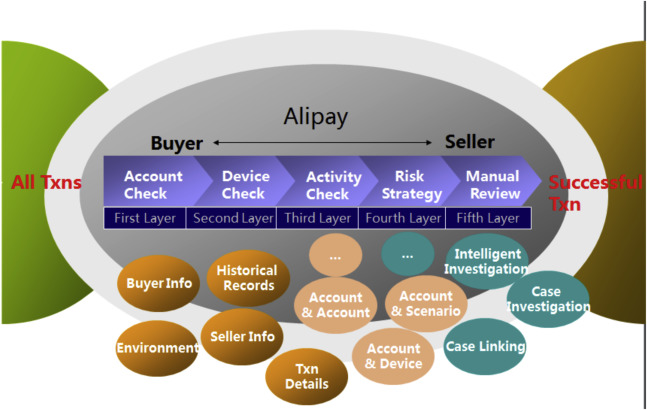
\includegraphics[scale = 0.8]{figures/alipay.jpg}
	\centering
	\caption{Fraud analytics in Alipay}
	\label{fig:alipay}
\end{figure}

Stages of fraud restrictions :
\begin{itemize}
	\item Account check
	\item Device check
	\item Activity check
	\item Risk strategy 
	\item Manual review
\end{itemize}

RAIN - model used by Alibaba stands for Risk of activity, identity and network~\ref{fig:rain_dimension}. It identifies the risk of any object interacting with the Alibaba system such as a human, credit card or account. 3 dimension are defined in the system viz., activity, identity and network; and all variables are classified into them, values of variables are computed for all the objects. Depending upon the scenario particular variables are chosen and RAIN score is computed. Such as in the case of credit card fraud, identity variables are adjusted with higher weights; in the case of credit scoring network group of variables are weighted more. Logistic regression part of a Machine learning is used to determine the weights for a given scenario.

\begin{figure}[H]
	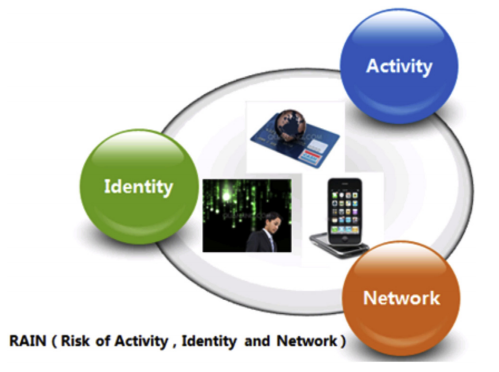
\includegraphics[scale = 0.8]{figures/RAIN_dimension.png}
	\centering
	\caption{Dimensions of RAIN score}
	\label{fig:rain_dimension}
\end{figure}

Network based graph representation is also used to link accounts and ip addresses to visually represent the links between name, address, phone, credit card, etc.

\chapter{Prescriptive Techniques}
\label{prescriptive-techniques}

A group of data analysis techniques which can suggest possible outcomes and prescribe recommendations and suggestions.
Prescriptive analytics is really valuable, but largely not used. According to Gartner, 13\% of organizations are using predictive but only 3\% are using prescriptive analytics. 
Big data analytics in general sheds light on a particular subject, but on the other hand prescriptive analytics answers specific questions with laser-like focus. 
Generally the techniques are used to optimize output, schedule and manage inventory for supply systems

\section{Game theory}
\label{game-theory}
This is a technique for analyzing the end result by the study of conflict and co-operation of the independent agents. Agents may be groups or individuals or a combination of these. Game theory came into existence in 1944 when John van Neumann \& Oskar Morgenstern published \textit{``Theory of Games and Economic Behavior``}.
Game theory has been successfully applied to design of auctions. 
United states raised billions of dollars by allocating resources more efficiently with auctions designed with Game theory, compared to the ones allocated by traditional auctions.
Automated decision making processes have been designed and modeled with game theory principles. 
%
%
%
%

\setlength{\footskip}{8mm}

\section{Optimization Techniques} 
\label{optimization-techniques}

%
%
%
%

\setlength{\footskip}{8mm}

\section{Simulation Techniques} 
\label{visualization-techniques}

In the paper title \textit{``Monte Carlo method in risk analysis for investment projects``}~\shortcite{platon2014monte}, the authors have studied the effect of random input values to the possible outcomes for risk assessment of environmental projects. The Monte carlo model is evaluated with a random input from a normal probability distribution and the output. 
Monte carlo simulation was formulate around 1944. The method is used to produce artificial values for a probabilistic variable by the use of:
\begin{itemize}
	\item a random uniformly-distributed number generator in the $ [0,1] $ interval, and
	\item a cumulative distribution function associated with the stochastic variable
\end{itemize} 
There were three steps in the process of simulation. 
\begin{enumerate}
	\item Select an investment project
	\item Estimate risk of crossing value or cost of project
	\item Estimate risk of extension in implementation
\end{enumerate}
There exist alternate methods of plan and execution for risk mitigation :
\begin{itemize}
	\item risk acceptance or tolerance
	\item monitoring of process risk
	\item risk avoidance strategy
	\item mitigation and outsourcing
\end{itemize}

%
%
%
%

\setlength{\footskip}{8mm}

\begin{landscape}
	\chapter{Research literature summary}
In this section a summary of all the referred articles are presented in table~\ref{my-label}.

%\begin{table}[H]
%	\centering
	\hskip-5.0cm 
	\begin{longtable}[c]{|p{4cm}|p{6cm}|p{4cm}|p{6cm}|}
				\caption{Relevant papers referenced.\label{my-label}}\\
		\hline
%		\multicolumn{2}{| c |}{Begin of Table}\\
%		\hline
%		Title and Author & Data  & & \\
				\rowcolor[HTML]{000000} 
				{\color[HTML]{FFFFFF} \textbf{Title \& Author}} & {\color[HTML]{FFFFFF} \textbf{Objective}} & {\color[HTML]{FFFFFF} \textbf{Data}} & {\color[HTML]{FFFFFF} \textbf{Conclusion}} \\ \hline
%		\hline
		\endfirsthead
		
		\hline
%		\multicolumn{2}{|c|}{Continuation of Table \ref{long}}\\
%		\hline
%		Something & something else\\
				\rowcolor[HTML]{000000} 
				{\color[HTML]{FFFFFF} \textbf{Title \& Author}} & {\color[HTML]{FFFFFF} \textbf{Objective}} & {\color[HTML]{FFFFFF} \textbf{Data}} & {\color[HTML]{FFFFFF} \textbf{Conclusion}} \\ \hline
		\hline
		\endhead
		
%		\hline
%		\endfoot
		
%		\hline
%		\multicolumn{2}{| c |}{End of Table}\\
%		\hline
		\hline
		\endlastfoot
		``Social media big data and capital markets—An overview``~\shortcite{bukovina2016social}
		& Study capital markets relation to social media
		& 
		&
		\\ \hline
		``When machines read the news``~\shortcite{gross2011machines}
		& $\rightarrow$ To find if trading is news dependent,
		\newline $\rightarrow$ To find is intraday news affects high-frequency returns, volatility and liquidity, 
		\newline $\rightarrow$ To relate the market reaction to the relevant news broadcast
		& News data sourced from Reuters NewsScope Sentiment Engine, over 29k records of headlines 1 year interval from 2007-2008
		& It`s a challenging task since news is flooded by noise caused by irrelevant news items. 
		\\ \hline
		``Usage of location analysis software in the evaluation of commercial real estate properties``~\shortcite{droj2015usage}                                          & To assess the usefulness of Location analysis to determine the valuation of commercial property. Variables of assessment include proximity to schools, markets, main roads, rail and bus stations; pollution index of area; existence of public services like electricity, water, sewage, phone, heating etc.; access to additional services like education, health centers, leisure, recreation.
		& Cadaster information from city of Oradea, Romania.
		& Property value estimation can be evaluated accurately by integrating economic and building construction data to the spatial analysis data. Cadaster administration is used in conjuction with GIS to precisely estimate property values.
		\\ \hline
		``Applying Fuzzy Logic and Machine Learning Techniques in Financial Perfor-mance Predictions``~\shortcite{Costea2014}
		& obj
		&
		&
		\\ \hline
		``Artificial intelligence. McGraw-Hill, New`` ~\shortcite{rich1991artificial} 
		& obj 
		& data 
		& Conclusion
		\\ \hline
		``Deep learning in finance``~\shortcite{heaton2016deep}
		& obj
		& data
		& conclusion
		\\ \hline
		``Big
		data based fraud risk management at Alibaba.``~\shortcite{Chen2015}
		& obj
		& data
		& conclusion
		\\
		“Monte Carlo method in risk analysis for investment projects“~\shortcite{platon2014monte}
		& obj
		& data
		& conclusion
		\\
	\end{longtable}
	
%	\begin{tabular}{|p{6cm}|p{6cm}|p{6cm}|l|}
%			\hline
%		\rowcolor[HTML]{000000} 
%		{\color[HTML]{FFFFFF} \textbf{Title \& Author}} & {\color[HTML]{FFFFFF} \textbf{Objective}} & {\color[HTML]{FFFFFF} \textbf{Data}} & {\color[HTML]{FFFFFF} \textbf{Conclusion}} \\ \hline
%		``When machines read the news``~\shortcite{gross2011machines}
%		& $\rightarrow$ To find if trading is news dependent,
%		\newline $\rightarrow$ To find is intraday news affects high-frequency returns, volatility and liquidity, 
%		\newline $\rightarrow$ To relate the market reaction to the relevant news broadcast
%		& News data sourced from Reuters NewsScope Sentiment Engine, over 29k records of headlines 1 year interval from 2007-2008
%		& 30 \\ \hline
%		``Usage of location analysis software in the evaluation of commercial real
%		estate properties`` ~\shortcite{droj2015usage}                                          & obj                                       & 20                                   & 30        \\ \hline
%		``Applying Fuzzy Logic and Machine Learning Techniques in Financial Perfor-
%		mance Predictions`` ~\shortcite{Costea2014}                                          & obj                                       & 20                                   & 30         \\ \hline
%		``Artificial intelligence. McGraw-Hill, New`` ~\shortcite{rich1991artificial} & obj & data & Conclusion\\ \hline
%	\end{tabular}%
%	}

%	\caption{Literature review summary table}
%	\label{my-label}
%\end{table}
\end{landscape}

%\setlength{\footskip}{8mm}

\chapter{Literature Review} 
\label{ch:literature-review}

This thesis chapter introduces concepts, technologies, techniques, consulted papers and articles pertaining to the core concepts of Customer Churn \& Retention, OLAP \& Datawarehouse, Data mining, Model evaluation metrics, Review of of selected papers and Summary of selected papers.

\section{Customer Churn \& Retention}
Customers are the most volatile asset of a services based company. Many frequently churn in search of better services. Customers are frivolous and those with prepaid or prepay plans are most unfaithful. Companies are generally in profit if they are able to retain customers and it pays off to almost six times \shortcite{bhatt1998custret}. Customers spending longer durations with a company are not easily churned and would not be affected by marketing strategies of rival companies. These customers are valuable to the company and generate profit in revenue. Research studies  have shown that long standing customers would be engaged in influencing newer customers to buy into a contract with their service provider \shortcite{mizerski1982}.\\
The ARPU of a stable customer is high compared to that of a churning customer. Thus marketing managers are focusing on advertising competitive products to retain customers from churning. The loss of capital due to a defecting customer is higher than the cost of retention. As per Forbes, Nov 11, 2013, earnings can swing positively by about 10 \% if customers are successfully retained.

\section{OLAP \& Datawarehouse }
Systems and companies are ever expanding. They are collecting data at unprecedented rates. Managing data becomes easier with the implementation of Data-warehouse. In many a cases the database of a company is segregated into different schema's. Segregation of schema's helps to avoid necessary access privileges and grants confusion. It also helps to maintain the organizational level of segregation in the database, ie., the HR department tables will be unaccessible to an accounts official and vice versa. But company leaders and decision makers should be accessing specific key counts and aggregations from all of their departments. A collection of tables sourcing data from their individual units.\\

OLAP - Online Analytical Processing is an extension of Data-warehouse technology \shortcite{han1997olap}. Olap consists of four main processes viz., Drill-down, Roll-up, slice and dice. Multi-demensional data can be fetched by OLAP from the Datawarehouse, and the unit of this is called the OLAP cube.There are two types of OLAP - MOLAP \& ROLAP. MOLAP Multidimensional OLAP is a solution used widely. 

One very famous open-source  OLAP solution is the Kylin\textsuperscript{TM} \shortcite{ApacheKylin}. Shown in Figure~\ref{fig:Kyline} is the architecture of the product.


\begin{figure}[h]
	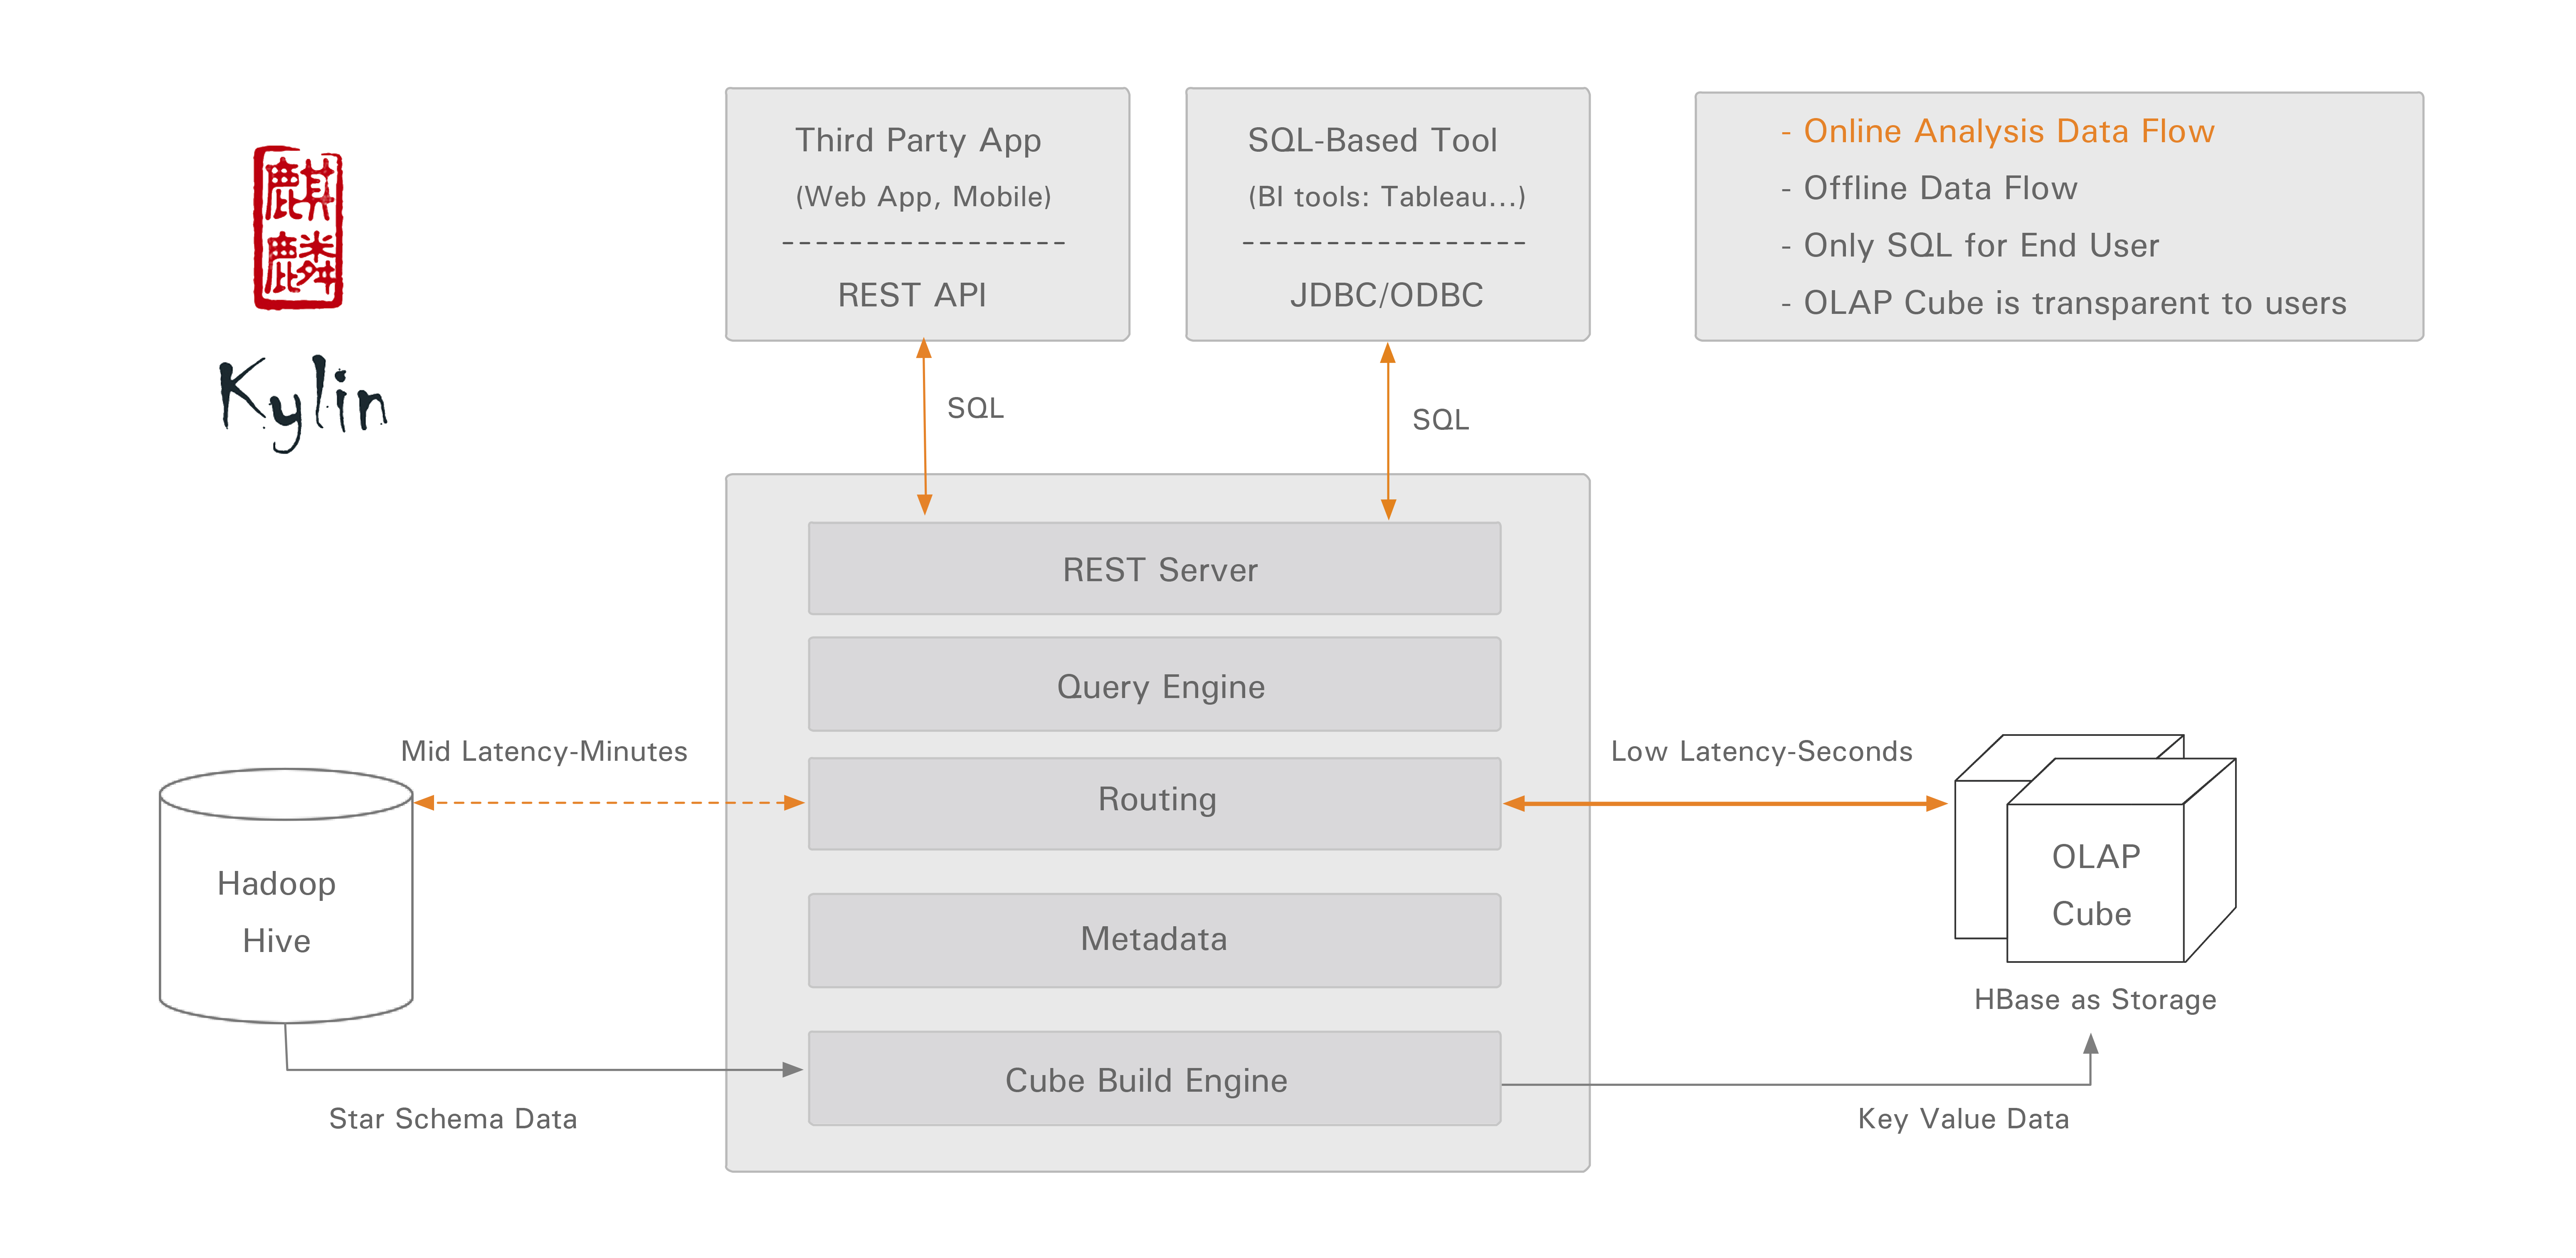
\includegraphics[width=\columnwidth,height=9cm]{figures/kylin_diagram.png}
	\centering
	\caption{OLAP Solution - Apache Kylin}
	\label{fig:Kyline}
\end{figure}


\section{Data Mining}
\label{data-mining}
Data mining is the process of extracting useful trend and patterns from structured and unstructured sources of data. Sometimes many academicians refer to it as KDD (Knowledge Discovery in Databases). John Naisbett (author of famous 'Megatrends') said \say{We are drowning in information but starved for knowledge.}
There are various techniques to perform data mining and these can be broadly classified into two categories Supervised Learning, Un-Supervised Learning.	
A very common terminology used in the data science field is of machine learning and it also used instead of data mining. 

\subsection{Supervised Learning}
This part of the data mining consists of classification and regression algorithms. Control and dependent variables of the given data are known entities. The use of these algorithms is to predict the outcome given past data. These algorithms have to be trained with a set of data and then they have to be tested. After reaching certain acceptable level of accuracy, these algorithms are used for prediction. 
\\
\\
Below are some of the Supervised learning techniques :
\begin{itemize}
	\item Linear regression : The prediction of dependent variable is done given the value of known variable. There is only 1 dependent variable. For example, \(y=\beta0 + \beta1x + \varepsilon\) \\
	y = dependent variable, 
	x = independent variable
	\item Multiple regression : is an extension of the linear regression but has more number of independent variables.
	\item Nonlinear regression : there are two variables but they are related in a curvilinear fashion i.e., not governed by the straight line equations.
	\item Logistic regression : A regression based modeling technique, which is better than linear regression when more variables are considered. Output variable is categorical in nature. 
	\item Decision tree : This is a classification algorithm which when plotted resembles an upside down tree structure. Given that a set of data has many attributes and there is a need to classify them, a decision tree is very suitable method to do so. There are many types of decision trees like the ID3, CART, C4.5 and C5.0. In Figure~\ref{fig:decisiontree} a simple DT for mammal classification model is shown. A decision tree can be designed using \textbf{Hunt's Algorithm}.
	\begin{figure}[H]
		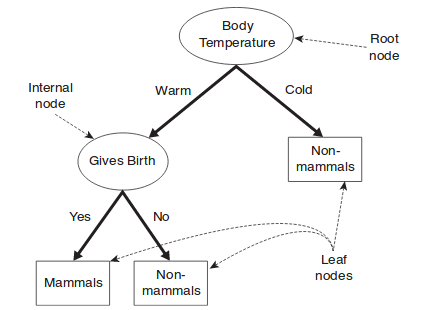
\includegraphics[scale=0.65]{figures/example_decisiontree.png}
		\centering
		\caption{Mammal classification problem}
		\label{fig:decisiontree}
	\end{figure}
	\item Random Forest : This technique can be used for both classification or regression type problems. A random forest is combination of many decision trees. In some cases random forest is sometimes very accurate.
	\item Support Vector Machine : This is a classifier technique where the data is segregated by generating hyperplanes. If there are n-features in the data then there have to be n-hyperplanes. The best classification is the hyperplane which clearly separates the data points.
	\item k-Nearest Neighbors : A learning algorithm that classifies the data into clusters nearest to them. The euclidean distance or manhattan distance could be some of the methods to find the nearest cluster. It is sometimes considered a lazy learning algorithm.
	\item Naive Bayes : This is an classification rule working on the probabilistic Bayes theorem.\newline
	 \(P(H|X) = P(X|H) P(H)/P(X)\).\newline
	\item Artificial neural networks : Neural networks are classification methods modeled after neurons \shortcite{neuralnetwork}. There are many layers with nodes Figure~\ref{fig:neuralnet}. There are many types of neural networks viz., Feed Forward NN, Radial Bias function, Recurrent NN, Backpropagation NN, Perceptron etc. Neural networks are very fast learners.
	\begin{figure}[H]
		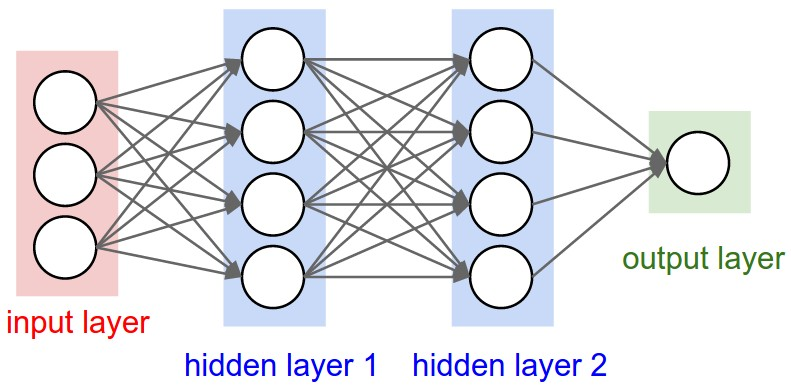
\includegraphics[scale = 0.5]{figures/neural_net2.jpeg}
		\centering
		\caption{A sample neural network}
		\label{fig:neuralnet}
	\end{figure}
\end{itemize}

\subsection{Un-Supervised Learning}
The clustering and association techniques in data mining are grouped into Un-Supervised learning. The output variables are not known.
Below are some Unsupervised class of algorithms :
\begin{itemize}
	\item K-means clustering : it is a means of clustering a set of data points with some k centroids. For each data point the distance is calculated and the nearest centroid is chosen and data point is associated with that cluster. After every iteration of cluster formation a new centroid is calculated and the distance of the data points are taken. The clusters are reformed and the iteration is performed till no data point movement happens.
	\item Apriori clustering : Here in the A priori algorithm is used to create the clusters. A priori is used for frequent item set mining states that sets of items are frequent if the items themselves are frequent. 
	\item Hierarchical clustering : This is a clustering method in which large clusters are further segregated into smaller clusters. This is the Divisive type of HC. In the Agglomerative type of HC, the nearby clusters are joined to form larger clusters. A Dendogram is used to graphically represent the clusters.	
	\item Hidden Markov models : These are used to analyze or predict time series problems in fields of speech, language, medicine, and robotics. Core of the technique is formed on the foundations of Bayes Network. In a markov chain a future state depends only on the current state. It is called Hidden because only certain measurements can be see of the states, not the states itself. Particle filter and Kalman filter are HMM's.
	\item Self organizing maps (SOM) : This is a type of neural network. Types are of Vector Quantizer or Kohonen SOM. In Figure~\ref{fig:kohonen} is an illustration of an Kohonen SOM.
		\begin{figure}[H]
			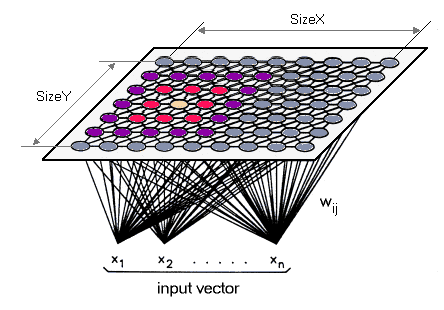
\includegraphics[scale = 1]{figures/Kohonen.png}
			\centering
			\caption{Kohonen SOM}
			\label{fig:kohonen}
		\end{figure}
\end{itemize}

\newpage
\subsection{Selecting the Right technique}
It is of utmost importance that a data scientist select the important mining  technique. Of all the process involved in the knowledge discovery process, selection of algorithm is quite difficult. Figure \ref{fig:selectdatamining},  from ``Choosing the Right Data Mining Technique: Classification of Methods and Intelligent Recommendation''  \shortcite{gibert2010choosing} shows the approach which could be taken to select between the various models available for data mining.

\begin{figure}[H]
	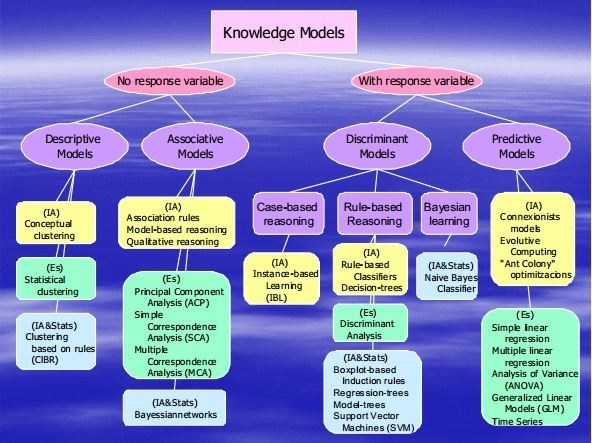
\includegraphics[width=\columnwidth,height=10cm]{figures/selectionofdatamining.jpeg}
	\centering
	\caption{Select the Right Mining Technique }
	\label{fig:selectdatamining}
\end{figure}

In addition to the above there is another approach, shown in Figure \ref{fig:scikit} suggested by the very popular scikit (machine learning library) of python for data mining \shortcite{scikitpython}.

\begin{figure}[H]
	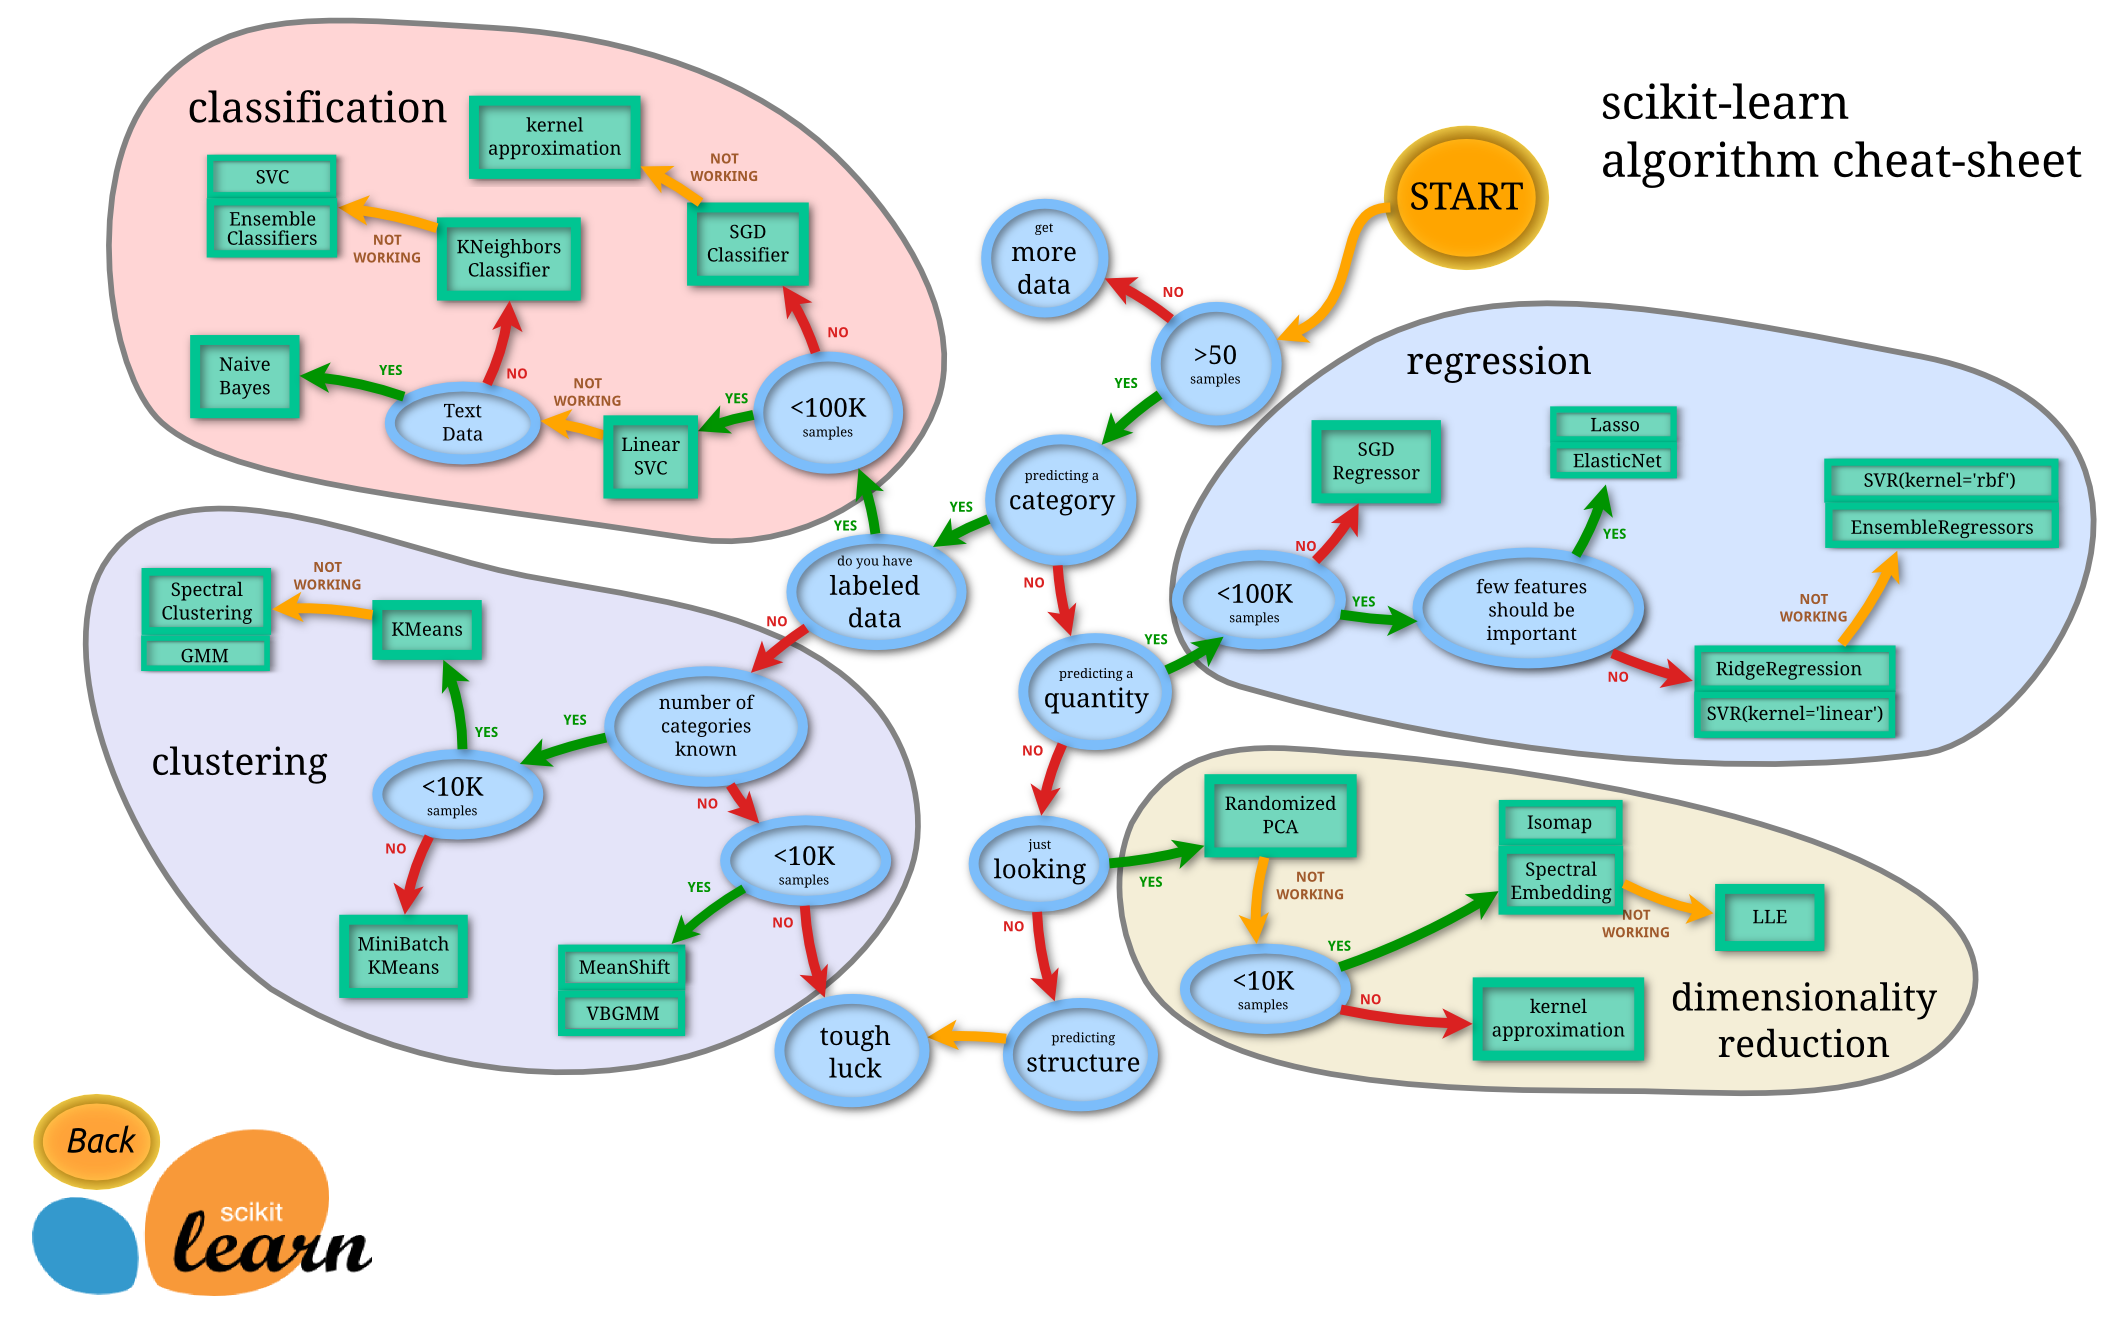
\includegraphics[width=\columnwidth,height=12cm]{figures/scikitlearn.png}
	\centering
	\caption{Another approach to select the Data Mining. Reprinted from Scikit}
	\label{fig:scikit}
\end{figure}


\subsection{Softwares, Libraries and Servers} 
Data mining techniques have been implemented into modules by a number of generous  contributers. There are some very famous solutions that an academician can utilize for implementing predictive analytics. The algorithms and techniques of neural networks, clustering, classification ans associations are available as solutions and API's. Following is a list in no particular order:
\begin{itemize}
	\item Softwares : The following softwares are open source and available for data analytics by downloading to the desktop.
	\begin{itemize}
		\item Weka : This is a open source software containing data mining algorithms. This can be used as a software or called by users own Java code.
		\item Knime : An open source tool for data mining, comprises of many functions from data cleaning to pattern analysis.
		\item Rapidminer : Also another popular tool for machine learning with plenty of algorithms for analysis.
	\end{itemize}
	\item Libraries : These are available for use as toolbox and academic can program own solution.
	\begin{itemize}
		\item Tensorflow
		\item mlpack
		\item H2O
		\item Mlib
		\item Scikit
	\end{itemize}
	\item Servers : The following servers have built in modules that can be accessed via web applications and can be modeled to process real time analytics instead of one of processing as with above solutions
	\begin{itemize}
		\item \textbf{DeepDetect} : is an open source deep learning server implemented in C++. It can be supported with back end machine learning applications with TensorFlow XGBoost and Caffe. Model assessment is built in the framework.
		\item \textbf{Apache Prediction IO} : This a open source stack for academicians to deploy machine learning. The stack has an Event Server that can be used to query from a web application and respond in real time. The Event server co-ordinates with the Engine to respond to API inputs and respond with predicted outcomes Figure \ref{fig:predictionio} \shortcite{PredictionIO}. PredictionIO provides various templates for varied mining algorithms. Classification templates like Decision trees, Logistic Reressiong, NLP are available for use.
		\begin{figure}[H]
			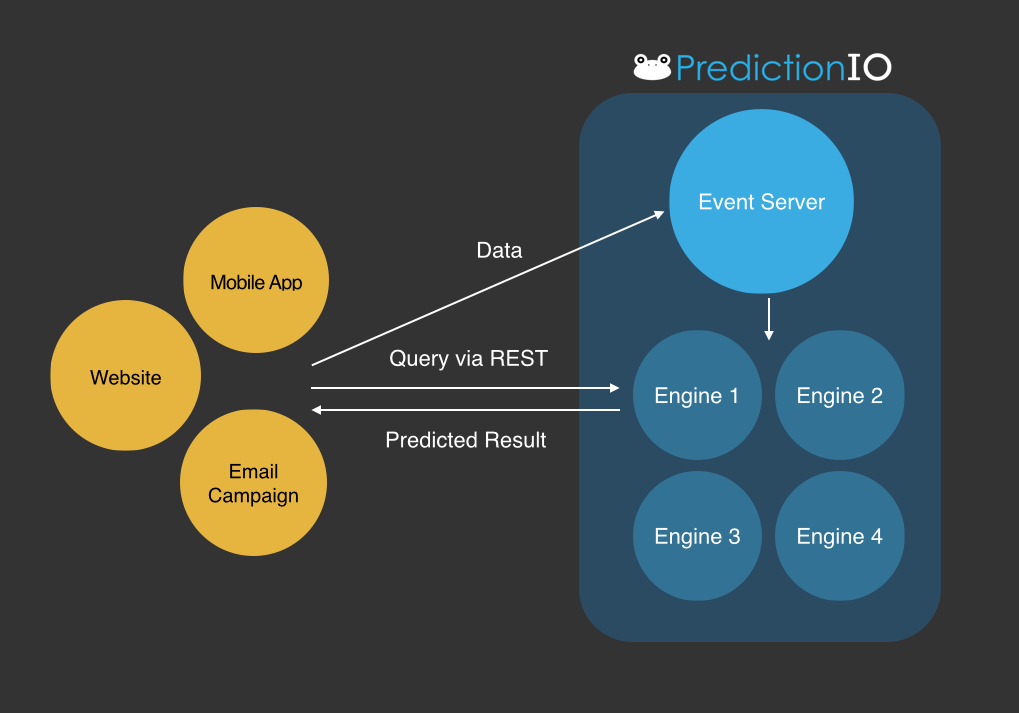
\includegraphics[scale=0.3]{figures/predictionioeventsever.png}
			\centering
			\caption{PreditionIO Engine interaction with Apps and Prediction Engine}
			\label{fig:predictionio}
		\end{figure}
		\item \textbf{Shiny} : This is an R package and allows for easy to build web applications. It is made of two parts UI script and server script. In Figure it can be seen how Shiny can be implemented to exploit the data mining capabilities of R. Shown in Figure \ref{fig:shinyscaling} how multiple users can access shiny R applications \shortcite{Rshiny}.
		\begin{figure}[H]
			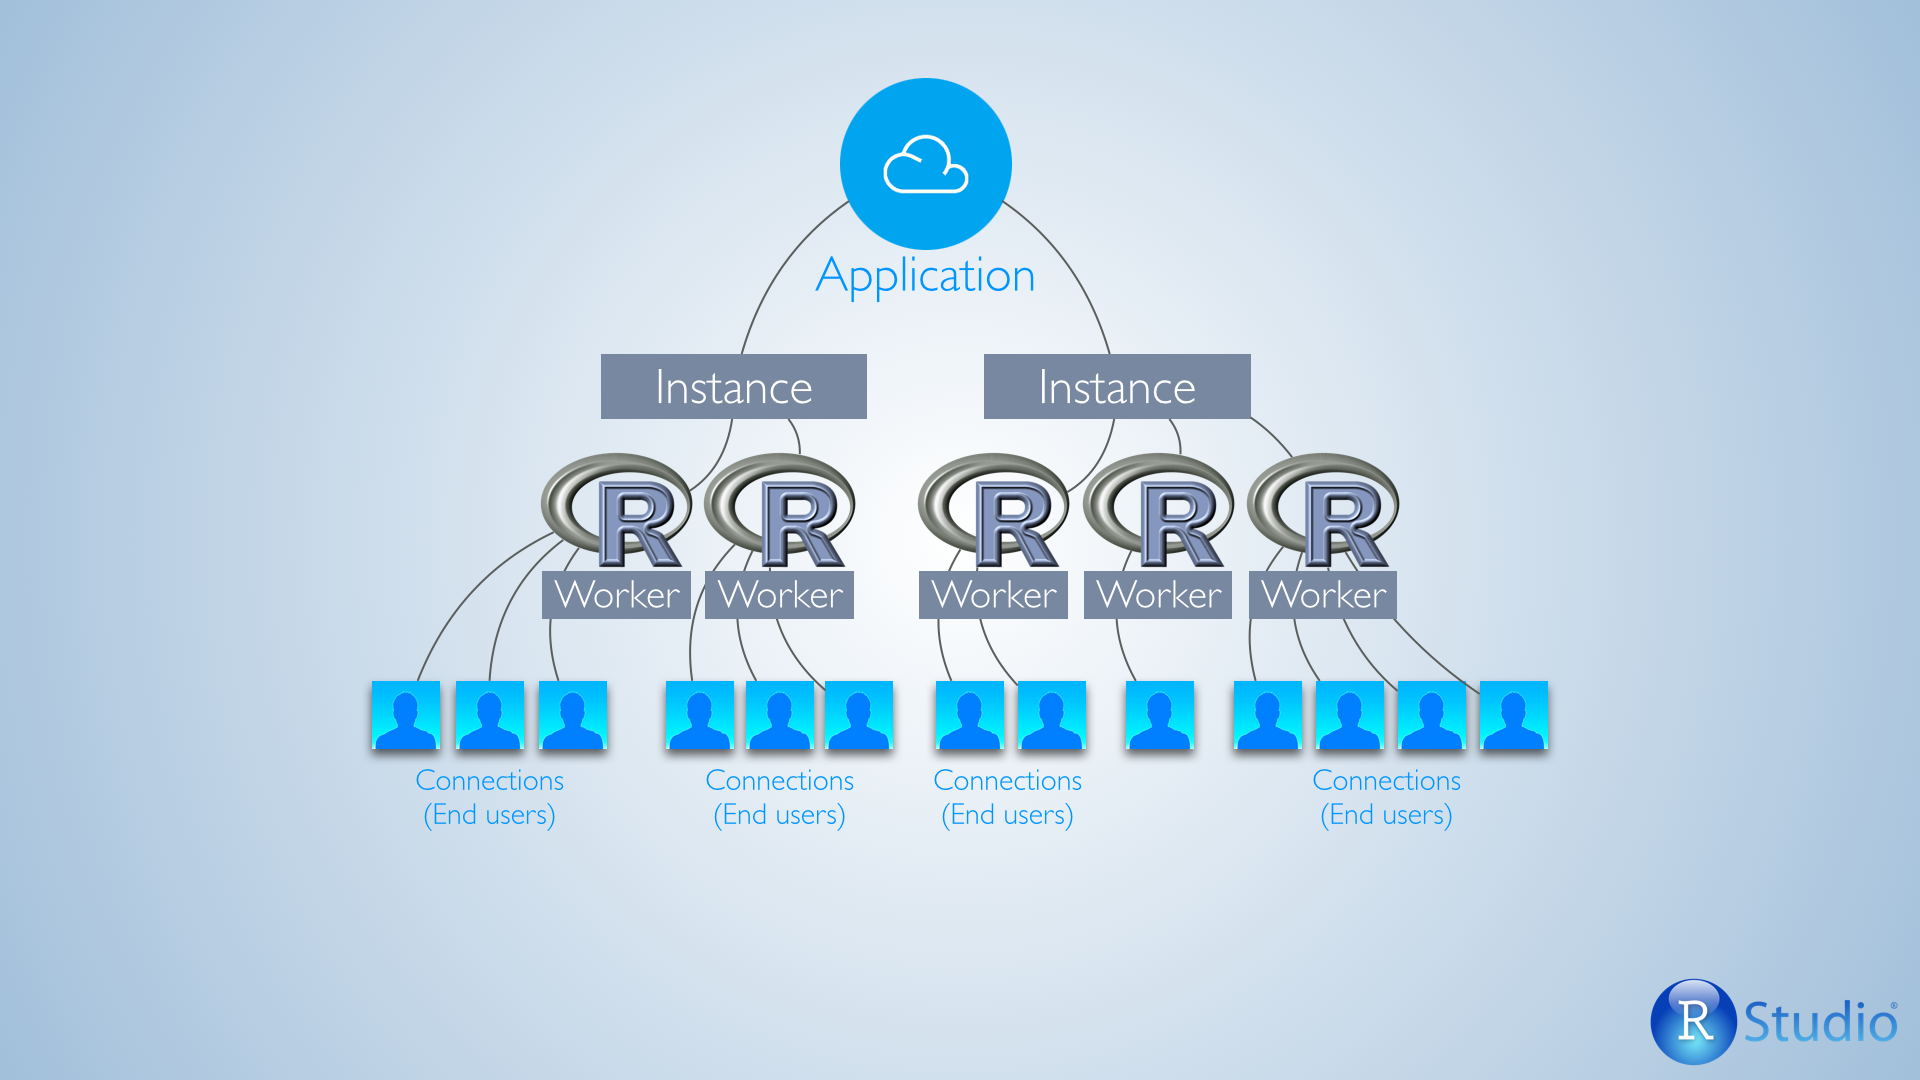
\includegraphics[width=\textwidth,height=10cm]{figures/shinyscaling.png}
			\centering
			\caption{R Shiny architecture}
			\label{fig:shinyscaling}
		\end{figure}
	\end{itemize}
\end{itemize}

\newpage
\section{Model Evaluation Metrics}
Model development is an important process, but evaluations of the model to ascertain its performance is as much an important procedure. The dataset is partitioned suitably and the testing set is not in the view of the model during training. There are however two methods of evaluations.

\begin{itemize}
	\item Holdout technique
	\item K-fold Cross validation technique
	\item Leave one out CV
	\item Bootstrap method
	\item Sensitivity \& Specificity
\end{itemize}

\subsection{Holdout technique}
This method is chosen for evaluation if the dataset is large enough. The data is segregated into three parts viz., Training, Validation and Test sets. 
\begin{itemize}
	\item Training dataset : It is some part of the dataset used for training the models. Predictive models are necessarily trained before actual prediction can be performed eg., Decision Trees, Random forest, Neural network need to be trained.
	\item Validation dataset : This is a subset of the data used to validate the output after model training. It helps to optimize the models performance. It is not mandatory to have validation sets for certain prediction models.
	\item Test dataset : Also a part of the whole dataset, it helps to  
\end{itemize}

\subsection{k-fold cross validation technique}
This method of evaluations is chosen if the dataset is small and limited. The data is partitioned into k equal sized sets with an unbiased process. The model is built k times, with every K-1 data sets selected as training set, leaving out 1 set to be used as test set. A round robin process is followed to select the testing set in every iteration.


\subsection{Sensitivity \& Specificity}
For calculating the performance of the model, a confusion matrix is plotted. The matrix is a cross table between predicted values and the actual values Figure \ref{fig:ConfusionMatrix}.  There are generally four types of values that can be calculated from the matrix and those are as follows :
\begin{itemize}
	\item TP - true positives : The predictor predicts ``True'' for actual true value of data. 
	\item TN - true negatives : The predictor predicts ``False'' for actual false values of data. 
	\item FP - false positives : The predictor predicts ``False'' for actual true value of data.
	\item FN - false negatives : The predictor predicts ``True'' for actual false values of data.
\end{itemize}

\textbf{Sensitivity :} the ratio of the count of the True Positives to the total count of events. This is also called the \textit{\textbf{Recall}}.
\[
	Sensitivity(or Recall) = \frac{TP}{TP+FN}
\]
\\
\textbf{Specificity :} the ratio of the count of the True Negatives to the total count of non-events.
\[
Specificity = \frac{TN}{FP+TN}
\]

In addition to the above, True Positive value is called the \textit{\textbf{Precision}}. 

Form the values of \textit{Precision} and \textit{Recall} another statistical measurement called F-score can be derived.
\[
	F = 2 \times \frac{precision \times recall}{precision + recall}
\]

\begin{figure}[h]
	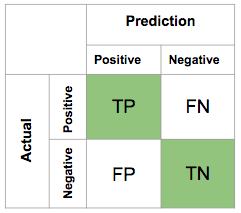
\includegraphics[scale=0.7]{figures/confusionmatrix.png}
	\centering
	\caption{Confusion Matrix}
	\label{fig:ConfusionMatrix}
\end{figure}




\newpage
\section{Review of Selected Research Papers}

In the paper titled `` Modeling \& Simulation  of a Predictive Customer Churn Model for Telecommunication Industry‘’ the authors emulated a neuro fuzzy inference system to study the customer churn in the telecom industry \shortcite{O2015}. They modeled membership functions for the attributes of the dataset. Then they employed search algorithm for feature selection of the variables that indicate churn. Thereafter they model fuzzy equations to relate the dependent variables to the independent variables. This fuzzy system is trained to tune the Adaptive neuro fuzzy system based on the Sugeno FIS. The call detail records of 5000 subscribers was used to model this FIS. The dataset has 21 attributes but here they selected 9. Then the variables were modeled into three categories. For performance evaluation they calculated the Precision rate and the recall rate. After the testing it was found that accuracy was 95.8\% , precision 80.86\%, recall 92.7\%.

A research study ``A Hybrid Churn Prediction Model 
in
Mobile 
Telecommunication Industry '' \shortcite{olle2014hybrid} presents a combination of LR and VP method. The academics used two algorithms of supervised learning viz., Logistic regression and Voted perceptron. They then combined the two into a Hybrid model for classification in WEKA.
The obtained the data from an Asian telcom operator, records of around 2000 customers and 23 attributes.\\
From the results it was observed that hybrid model performed better than each of them individually.

In the study ``A comparison of machine learning techniques for customer churn prediction'' by \shortcite{vafeiadis2015comparison} the researchers present a well meted out comparison between the normal model functions and their corresponding boosted models. The performance criteria was based on the F-score. They had used a series of simulations based on the Monte Carlo method. The models selected for analysis were Back-Propagation algorithm , Support Vector Machines, Decision Trees, Naive Bayes and Logistic Regression. The data was obtained from the publicly available churn dataset hosted at UCI Machine learning repository. The 100-fold cross validation technique was used to reduce bias. Ratio of training to testing set is about $2:3$. A type of the most common boosting algorithm Adaboost, \textit{Adaboost.M1} with DT and BPN as weak classifier was used.\\
The R programming was used for modeling the simulation experiment. Two steps were followed : Step 1 - tested classifiers run with data and performance of F-score measured. Step 2 - boosting algorithm was applied and performance F-score measured. 100 Monte carlo realizations were generated for cross validation of results. Monte carlo is synthesis of datasets that resemble the actual data. It was derieved from the results that two prediction models performed the best. 2 layer BPN with 15 hidden nodes and Decision tree classifier. An accuracy of 94\% and F-measure around 77\%. The SVM scored lower followed by Naive Bayes and Logit Regression at last. After application of the Boosting algo, SVM reported the best accuracy of 97\% and Fmeasure over 84\%.


\begin{landscape}
\section{Summary of Selected Research Studies}
Here some of the past relevant literature in the domain of churn prediction and the results are discussed in Table \ref{table1}.

\begin{longtable}{ | p{20pt} | p{100pt} | p{100pt} | p{150pt} | p{100pt} | p{150pt} | }
	\caption{Previous literature review.}\label{table1}\\
 	
 	\hline
 	SNo & Title \& Author & Objective &  Data \& Methodology & Outcome & Further Research\\
 	\hline
 	\endfirsthead
 	
 	\hline
 	SNo & Title \& Author &Objective & Data \& Methodology &Outcome & Further Research\\
 	\hline
 	\endhead
 	\hline
 	\endfoot
 	\hline
    \endlastfoot
    \hline
    1    % .......................... New Entry
    &
    Modeling \& Simulation  of a Predictive Customer Churn Model for Telecommunication Industry \shortcite{O2015}
    &
    Adaptive neuro fuzzy inference system for prediction emulation of customer churn Neural network + fuzzy logic.
    &
    \textbf{Data :} 5000 subscribers CDR – call detail record with 21 vriables. Partitioned into 5 sets each containing 1000 records.
    \newline
    \textbf{Method :} Number of predictor variables taken is 9. Target variable is Chrun with value Y or N. Membership function for each variable.
    &
    Found that 3 variables are very important. 
    Total no of minute calls, no of customer service calls, no of repaired calls.
    Fuzzy churn model Precison 80.86\% recall 92.7\% and predicted accuracy 95.8\%.
    &
    None suggested
    \\\hline
    2    % .......................... New Entry
    &
    A Hybrid Churn Prediction Model in Mobile Telecommunication Industry \shortcite{olle2014hybrid}
    &
    A model combined with VotedPerceptron and Logisti Regression is performance compared to the models of VP and LR as individual predictors.
    &
    \textbf{Data :} 2000 customers CDR from an Asian telecom company with 23 attributes.
    \textbf{Method :} A hybrid model of VP and LR was used. WEKA tool was used to model.
    &
    The hybrid model performs better than the models prediction accuracy seperately.
    & None suggested
    \\\hline
 	  	 3    % .......................... New Entry
 	  	 &
 	  	 A comparison of machine learning techniques for customer churn prediction \shortcite{vafeiadis2015comparison}
 	  	 &
	  	 The normal model functions were performance compared to their corresponding boosted models.
 	  	 &
 	  	 \textbf{Data :} publicly hosted churn dataset at UCI machine learning repository.
 	  	 \newline
 	  	 \textbf{Method :} Machine learning techniques of Back-Propagation algorithm , Support Vector Machines, Decision Trees, Naive Bayes and Logistic Regression were used. The boosting algorithm Adaboost.M1 a type of Adaboost was used. R progamming was used for modeling the system.
 	  	 &
 	  	 2 prediction models performed the best : 2-layer BPN with 15 hidden nodes and Decision tree classifier. SVM scored lower followed by Naive Bayes and Logit Regression at last. After application of the Boosting algo, SVM reported the best accuracy of 97\% and Fmeasure over 84\%.
 	  	 & None suggested
 	  	 \\\hline
 	 
 	 4    % .......................... New Entry
 	 &
 	 Turning telecommunications call details to churn prediction: a data mining approach \shortcite{wei2002turning}
 	 &
 	 The company experiences a high monthly churn rate of 1.5 – 2%. 
 	 Neural network requires a long time due to it’s iterative nature.
 	 Highly skewed class distribution between churners and non-churners.
 	 &
 	 \textbf{Data :} Telecom company of Taiwan. Contractual and call details of subscribers Oct 2000 – Jan 2001. 9100000 records.
 	 \newline
 	 \textbf{Method : } Multi classifier class combiner, Decision tree C4.5 
 	 &
 	 Churn prediction is relatively high within 1 month duration. Multi classifier performs better than single classifier. 
 	 &
     To include more variables from logs and complaints. Evaluation of empirical stats between customers from different geographic locations. Integration with data-warehouse for constantly learning behavior of customer. Research with other industry data from credit card to Internet service providers.
 	 \\\hline
 	 5    % .......................... New Entry
 	 &
 	 Applying Fuzzy Data Mining to Telecom Churn Management \shortcite{liao2011applying}.
 	 &
 	 To determine the most effective marketing strategies of customer retention, by analyzing the responses of customers. 
 	 &
 	 \textbf{Data :} Taiwan telecom company, retention activity \& response data for customer contract expiry between June and Junly 2008
 	 \newline
 	 \textbf{Method : } ID3 decision tree for classification.
 	 &
 	 Using fuzzy set the customer retention shows that marketing via telemarketing is more  effective compared with Direct mailing.
 	 Also fuzzy marketing technique is better than direct mailing marketing for customers with higher bill amounts.
 	 &
 	 Fuzzy data mining techniques to analyze the past records of results of various marketing activities to establish a marketing mode.
 	 \\\hline
 	 6    % .......................... New Entry
 	 & 
 	 Customer churn prediction using improved balanced random forests \shortcite{xie2009customer}.
 	 &
 	 a novel learning method, called improved balanced random forests (IBRF), and demonstrate its application to churn prediction
 	 &
 	 \textbf{Data :} Chinese bank data. 1524 [762 train, 762 test].
 	 \newline
 	 \textbf{Method : } IBRF = Balanced random forest + weighted random forest. 
 	 Introduce 2 interval variables ‘m – middle pt’ \& ‘d – length of interval’. 
 	 apply IBRF to a set of churn data in a bank as test the performance of our proposed method, we run several comparative experiments comparison of results from IBRF and other standard methods, namely artificial neural network (ANN), decision tree (DT), and CWC-SVM (Scholkopf, Platt, Shawe, Smola, \& Williamson,
 	 &
 	 Accuracy rate follows this pattern \(IBRF > CWC-SVM > ANN > DT\),
 	 Top-decile Lift varies as this \(IBRF > CWV-SVM > DT > ANN\).
 	 IBRF offers great potential compared to traditional approaches due to its scalability, and faster training and running speeds.
 	 &
 	 Experimenting with some other weak learners in random forests. Improving effectiveness and generalization ability.
 	 \\\hline
 	 7    % .......................... New Entry
 	 &
 	 Churn prediction in subscription services: An application of support vector machines while comparing two parameter-selection techniques \shortcite{coussement2008churn}
 	 &
 	 Churn prediction using SVM. Benchmarked to Logit regression and random forest.
 	 &
 	 \textbf{Data :} Belgian newspaper publishing  company. Training set 45000, Test set 45000
 	 \newline
 	 \textbf{Method : } Use of random forest software and SVM-toolbox. SVM compared to Logit regression \& random forest. 
 	 Grid search using 5-fold cross-validation
 	 &
 	 SVM trained on balanced distribution, outperforms logit regression when parameter selection applied. Random forest surpass SVM. Academincs and practionerx don’t need to rely on traditional Logit reg, SVM with parameter selection technique and random forest offer better alternative
 	 &
 	 No complete working meta-theory to choose kernel function and SVM parameters. Thus deriving a procedure to select proper kernel function and SVM parameter.
 	 \\\hline
 	 8    % .......................... New Entry
 	 &
 	 Customer churn prediction by Hybrid neural networks \shortcite{tsai2009customer}
 	 &
 	 Very few studies for hybrid data mining appraoch for prediction.
 	 &
 	 \textbf{Data :} CRM dataset from American telephone company, July 2001 to Jan 2002 51,306 subscribers.
 	 \newline
 	 \textbf{Method : } 2 methods developed and compared for performance. M1 – SOM + ANN clustering + classification is used. M2 – ANN + ANN 2 classifiers are used. 5 fold cross validation, each set of the 5 are tested 5 times. Baseline is 20 ANN’s
 	 &
 	 Baseline ANN models had prediction accuracy of 88\%
 	 performance : $ANN + ANN > single ANN$\newline
 	 $3*3$ SOM is best among $2*2$ , $3*3$, $4*4$ and $5*5$ clustering 
 	 Performance of the hybrid models is : $ANN + ANN > SOM + ANN > ANN$
 	 &
 	 Need to explore dimensionality reduction or Feature selection of data preprocessing. Application of SVM or genetic algorithms. Explore other domains for churn prediction.
 	 \\\hline
 	 9    % .......................... New Entry
 	 &
 	 Predicting customer retention and profitability by using random forest and regression forest \shortcite{lariviere2005predicting}
 	 &
 	 The paper discusses more than one variable of retention and profit outcome.
 	 &
 	 \textbf{Data :} 100,000 Belgian finance company. Divided into 2 random parts, one for estimation other for evaluation.
 	 \newline
 	 \textbf{Method :} Authors used random forest for regression to predict profitability,  next purchase and defection decision. Benchmarked to linear regression model.
 	 &
 	 Random forest are better than logit and linear regression.
 	 &
 	 None suggested.
 	 \\
 \end{longtable}

\end{landscape}

\begin{comment}

\section{Section Name in Literature Review}
\label{section-name-in-literature-review}

Example text below ..

\shortciteA{yamato92hmm} apply the background subtraction 
technique to extract blobs or human from a scene by the 
following conditions:
\[
\begin{array}{lc}
  {\rm if} & \left|{I_a (x,y) - I_b (x,y)}\right|< T,\;I_e (x,y) = 0 \\ 
  {\rm else} & I_e (x,y) = I_a (x,y), 
\end{array}
\]
where $I_e (x,y)$ is a human extracted image, $I_a (x,y)$ is an
original image, $I_b (x,y)$ is a background image, and $T$ is a
threshold. Figure~\ref{fig:mesh-feature} shows something. Some work also uses 
mesh features~\shortcite{yamato92hmm}.

% THE REASON ~ IS USED HERE BECAUSE WE TELL LATEX THAT THESE TWO WORDS SHOULD 
% GO TOGETHER IN THE SAME LINE.




\begin{figure}[t]
  \centering
  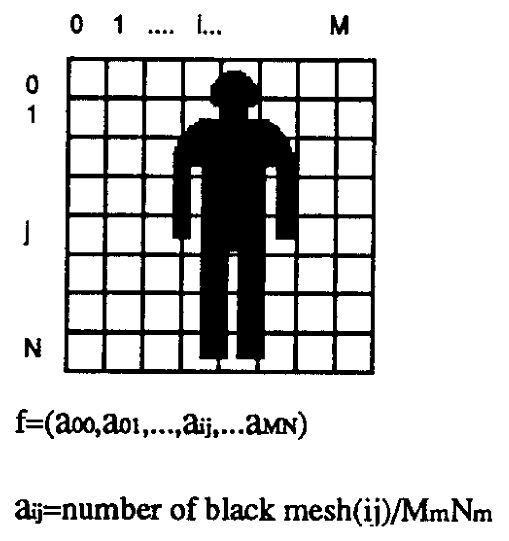
\includegraphics[width=2in]{figures/mesh-feature.jpg}  
  \caption[Mesh feature calculation]{Mesh feature
    calculation. Reprinted from the work of Yamato et al.\ (1992).}
  \label{fig:mesh-feature}
%\end{figure}

%/
\end{comment}


\FloatBarrier


%\setlength{\footskip}{8mm}

\chapter{Methodology}
\label{ch:methodology}

 In this chapter the methodology for implementing the ICPCR system is illustrated. Also the steps that would be followed are outlined.

\section{Research Methodology}
The following steps will be conducted also shown in Figure~\ref{fig:ResearchMethodology} :
\begin{enumerate}[label=Step \arabic*:]
	
	\item Data Preprocessing and Datawarehouse Development
	\begin{itemize}
		\item Data Collection
		\item Meta-data evaluation
		\item Data cleaning
		\item Datawarehouse design
		\item ETL process
	\end{itemize}
	\item Development and Evaluation of the Prediction Models
	\begin{itemize}
		\item Select three churn prediction models
		\item Models to be trained and tested with the data
		\item Model Evaluation
	\end{itemize}
	\item System Development \& Evaluation
	\begin{itemize}
		\item Build the ICPCR system as a web application.
		\item Integration of Web app with OLAP and prediction model.
		\item Develop the Dashboards to display KPI's.
		\item Test the system.
	\end{itemize}
\end{enumerate}

\begin{figure}[h!]
	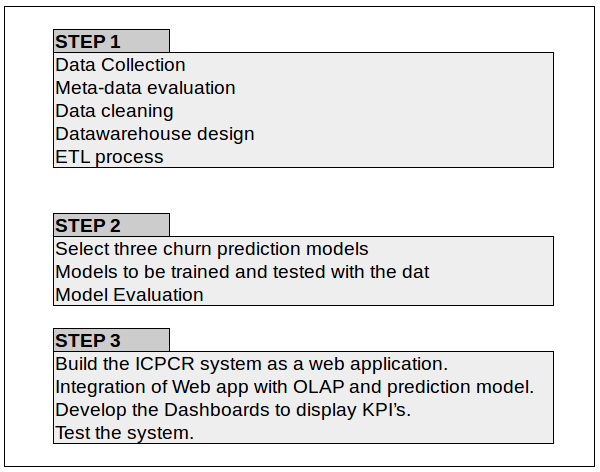
\includegraphics[scale = 0.5]{figures/ICPCR.png}
	\centering
	\caption{Research Methodology}
	\label{fig:ResearchMethodology}
\end{figure}
\newpage

\section{Data Preprocessing and Datawarehouse Development}

\subsection{Data preprocessing}

Data will be collected from available open source sites.
In this section a sequence of steps for data preparation are listed. In Figure \ref{fig:dataprerocessing} the process flow is shown.

\begin{enumerate}
	\item Study of meta-data of the dataset. This study reveals the important attributes to be used for prediction.
	\item Cleaning of un-usable data, either by replacing with suitable or by entirely removing it. Un-usable data is the one that may be invalid like null or special characters in numeric fields etc.
	\item Extract the data and load into the database. This helps in querying the data faster with Structured Query Language.
\end{enumerate}

\begin{figure}[h]
	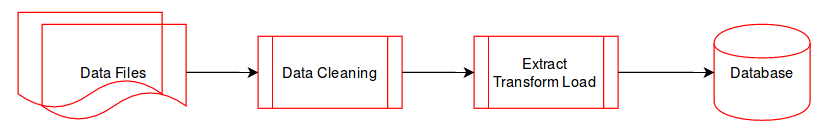
\includegraphics[scale = 0.5]{figures/dataloadprocess.png}
	\centering
	\caption{Data preprocessing}
	\label{fig:dataprerocessing}
\end{figure}


\subsection{Datawarehouse development}
Following steps will be followed for design of data warehouse:

The attributes generated from above step are summarized. This summary is used to design the OLAP cube. The OLAP will be used in generating reports and KPI's for the dashboard generation. The OLAP will be designed with the star schema. Figure~\ref{fig:olapstarschema} shows a typical implementation of the star schema \shortcite{olapstarschema}. A similar structure will be implemented for the study after the dimensions of the data are finalized.

Like for example the count of all the people between the age of 22 to 24 using prepaid service for the year 2013 could be one data whereas the count for 2014 would be another.

 \begin{figure}[h]
 	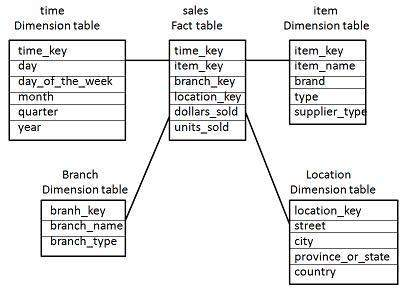
\includegraphics[scale = 0.7]{figures/olap_start_schema.jpg}
 	\centering
 	\caption{OLAP Star Schema}
 	\label{fig:olapstarschema}
 \end{figure}


After the Datawarehouse is designed, the tables have to be loaded with data. Thus the next step of ETL is done.
Extract Transform and Load processing (ETL) This is a necessary step that would be required to properly extract data from the data file, transform the data types in order that they may be suitable for the database and finally loading to database.
 
\newpage
\section{Development and Evaluation of the Prediction Models}
\subsection{Model Design}
In this section, the models are selected for churn prediction. Tentatively it is decided to select Decision tree, Support Sector Machine and ANN. The models will be trained with a training set and then the performance will be evaluated with the testing set. The proposal is to select either the machine learning library of MLib under Apache or Scikit of Python or libraries under R. It will largely depend on the availability of the models in the libraries. In case a model is not available it will be sourced from another library. Also in addition it is proposed that a boosting algorithm like Adaboost would be used to measure change in prediction performance.

\subsection{Model Evaluations}
In order to judge the better performing model or rather the accuracy of predictability by the classification techniques, it is but necessary to perform an evaluation. The evaluations that are commonly performed by academicians are the k-Fold Cross Validation, Sensitivity \& Specificity measurements \shortcite{lariviere2005predicting}.\\
\begin{itemize}
	\item K-Fold Cross Validation : It is proposed to per form this process to make the classification model more accurate. From previous literature it is learned that k = 100 is highly appropriate.
	\item Plotting of confusion matrix, as followed by other academicians and then deriving the Sensitivity, Specificity, Precision, Recall and F-score are the proposed evaluation techniques
\end{itemize}

\newpage
\section{System Development \& Evaluation}
In this section the architecture of the ICPCR system is proposed. The application, shown in Figure \ref{fig:system-design-churn-prediction}, would be developed in a 3-tire format i.e, Database Layer, Application Layer, and Presentation Layer. The system is designed in two modes. One is the learning phase mode and the other is the Prediction phase mode. In the learning phase the system is fed data and the inference engine learns the trend. Testing and benchmarking along with weighting.
\begin{figure}[h]
	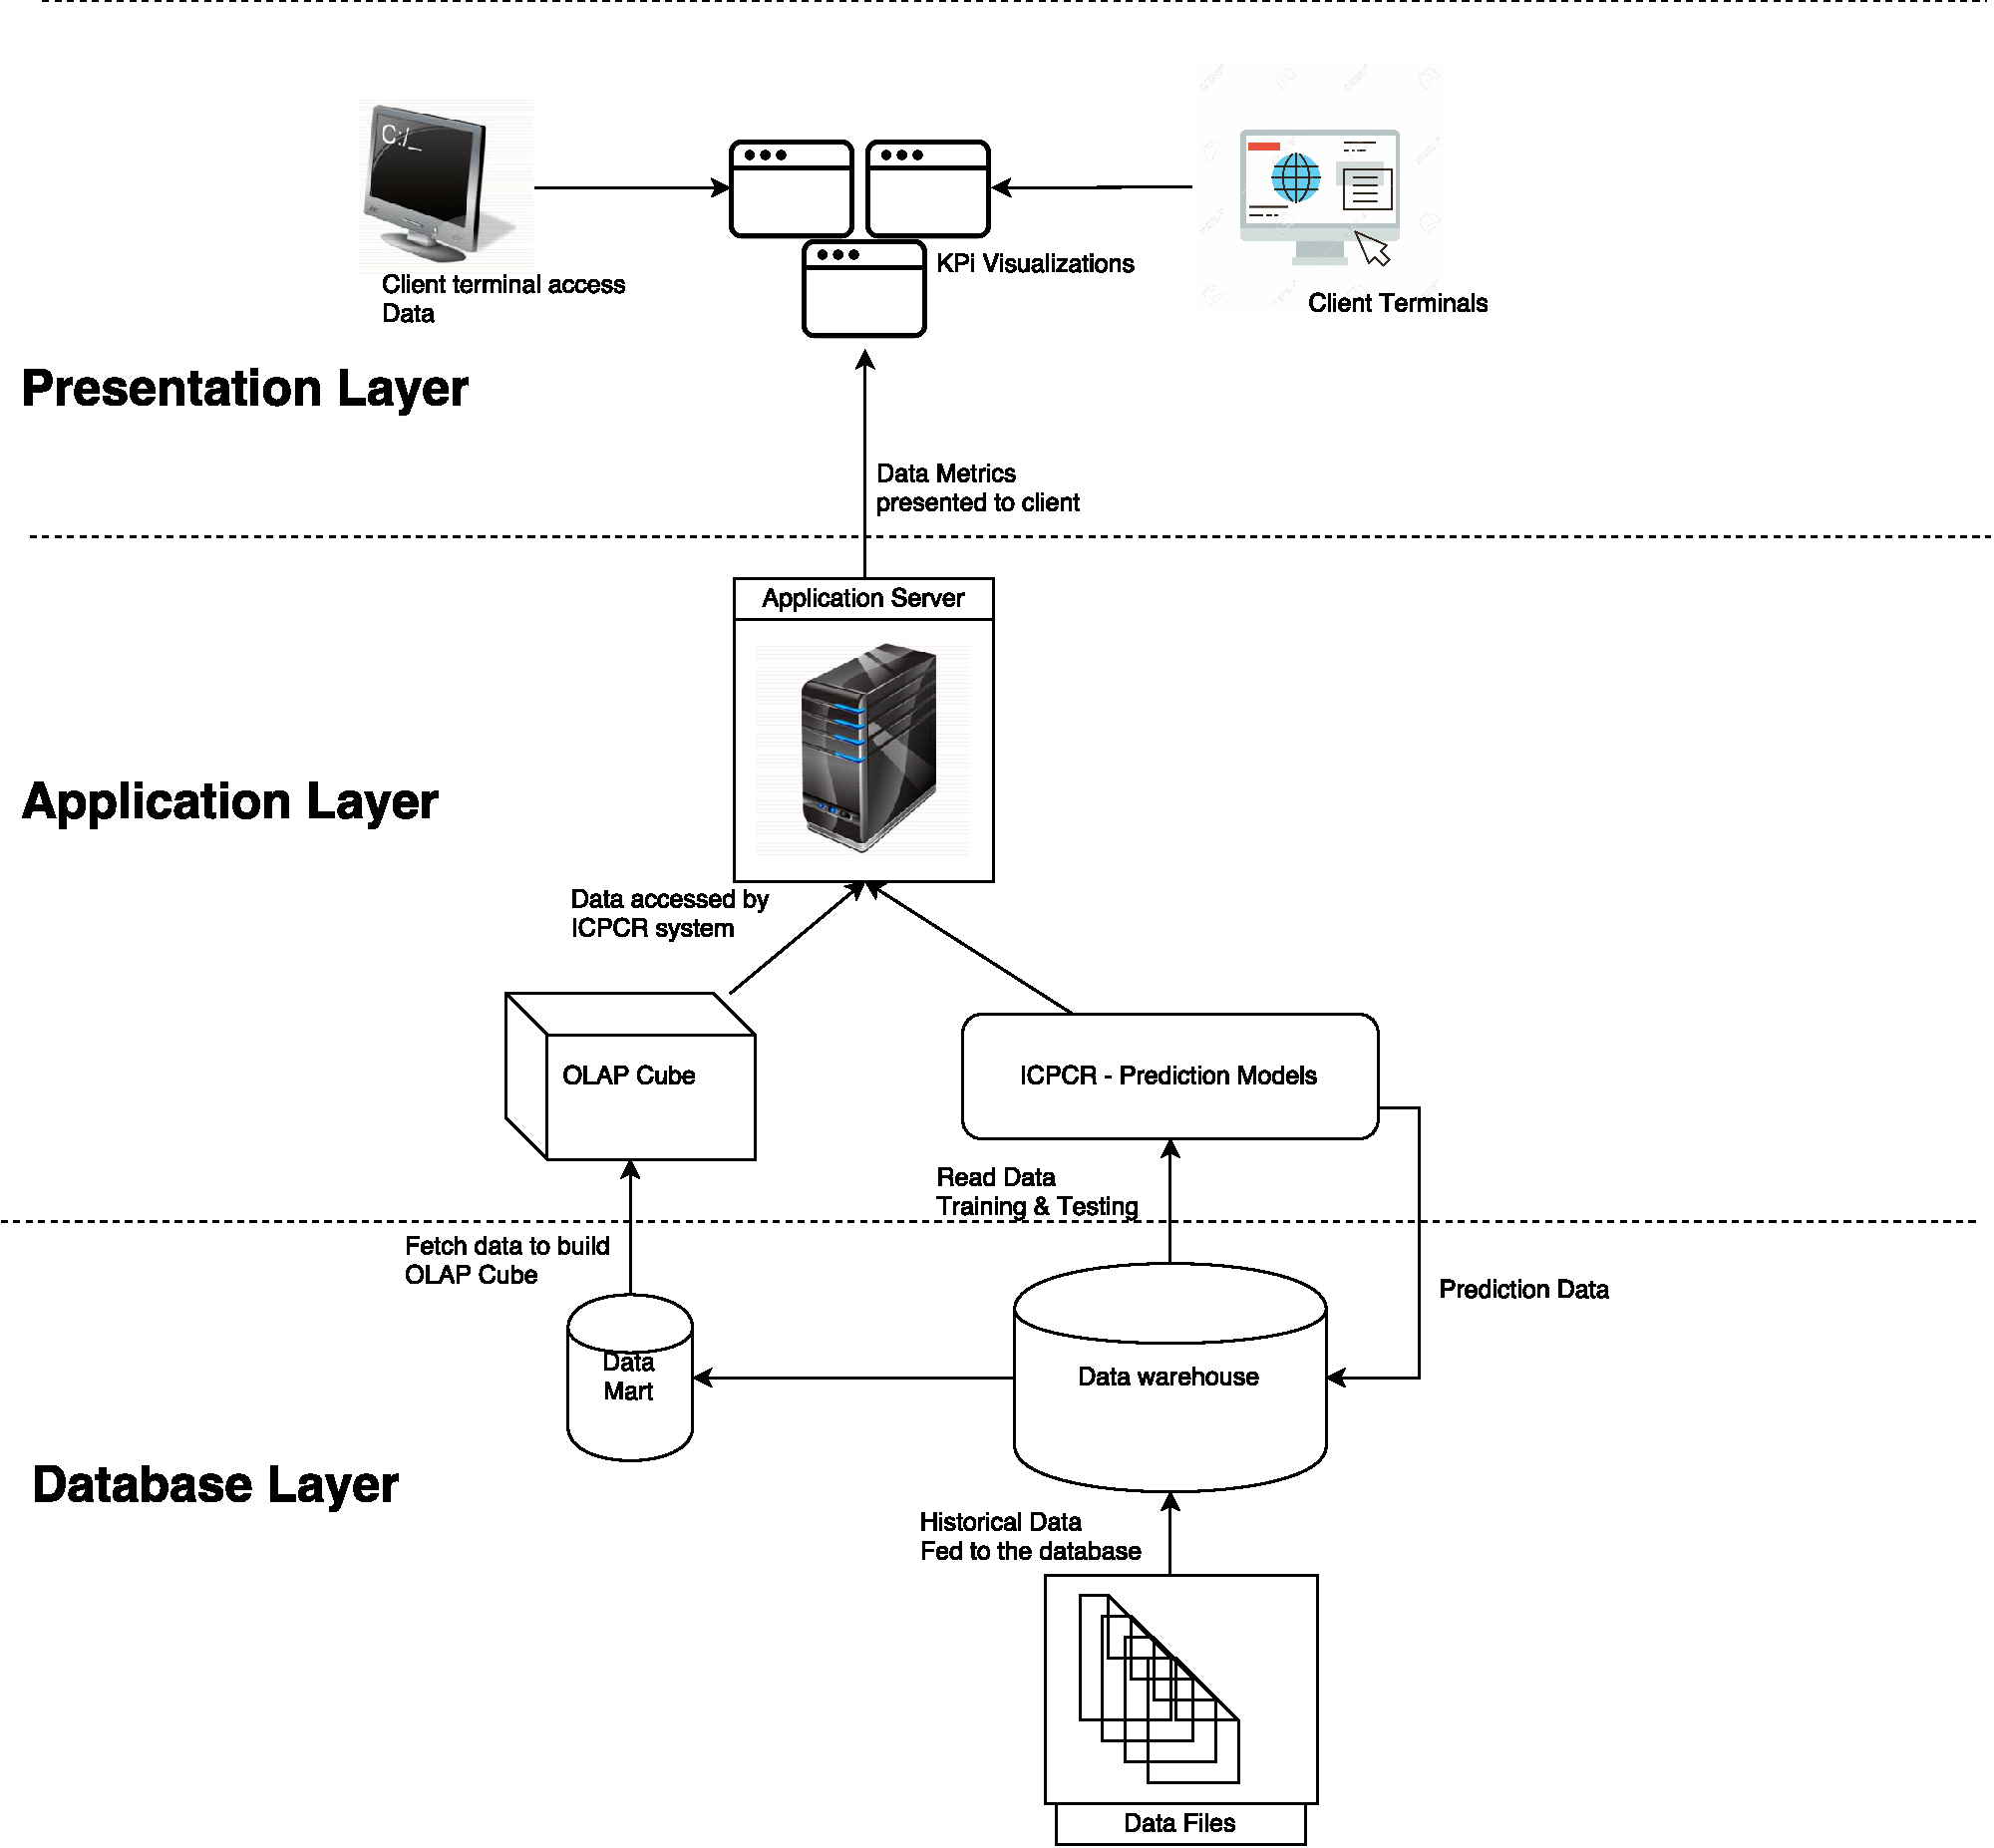
\includegraphics[width=\textwidth]{figures/ICPCR_pic1SystemDesign}
	\centering
	\caption{The Intelligent Churn Prediction Architecture}
	\label{fig:system-design-churn-prediction}
\end{figure}



\subsection{Presentation Layer}
In this thesis, the presentation layer is the section of the system which is accessible to the user or client. This is used to view the key values obtained from the OLAP and the mining results. There would be a display of metrics of the data.
\begin{enumerate}
	\item It is proposed to deploy a suitable application to display a dashboard of KPI's.
	\item The display of KPI's will be in graphs and charts format. The KPI's are taken from the OLAP cube.
\end{enumerate}


\subsection{Application Layer}
This layer would be comprised of three parts.
\begin{enumerate}
	\item Application server : This consists of the set of logic codes which will fetch the appropriate data for display in the front end. It may fetch the data directly from the tables or from the OLAP Cube, as is requested from the user.
	\item Prediction model : This part is comprised of the predictive model to predict the outcome of data presented to it in the database. The model will go through a phase of training, testing, and prediction of churn value for new data. Also it is proposed that Prediction model be able to identify the variables which could be addressed for retaining the customer.
	\item OLAP : This is the MOLAP implementation for building the Key metrics from the data. This part of the system would be responsible for the dashboard metrics display to the user.
\end{enumerate}


\subsection{Database Layer}
This layer will be comprised of the data-warehouse tables. The OLAP calculation and the Model predictions will be updated whensoever a set of ne data is identified. The Olap cube feed tables will also be present here. A Star schema will be implemented for fetching of data for the various dimensions of the OLAP.

\subsection{System Evaluation}
The thesis proposes a system evaluation process to audit the performance. A set of test from latency in display and run will be calculated and improved before the process of deployment. This would ensure that system does not behave erratically under normal situations.

\newpage
\begin{landscape}
\section{Timeline}
 The forecast of the tasks to be carried out in this thesis are shown below in a Gantt chart Figures~\ref{fig:time1}.
 \\
  \begin{figure}[H]
  	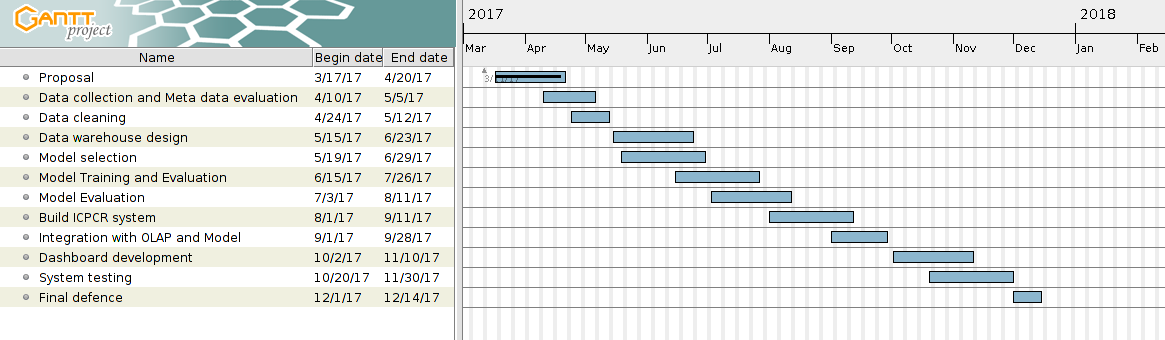
\includegraphics[width=25cm, height=10cm]{figures/churngantt3.png}
  	\centering
  	\caption{Gantt chart tasks}
  	\label{fig:time1}
  \end{figure}
\end{landscape}
% \begin{landscape}


%\begin{figure}[h]
%    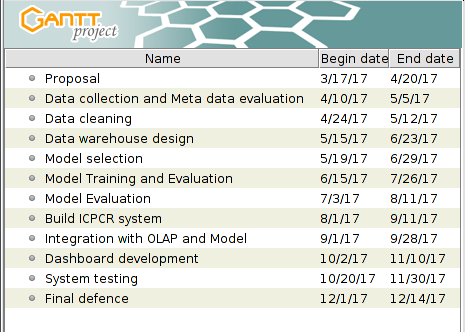
\includegraphics[scale=0.75]{figures/churngantt1.png}
% 	\caption{Gantt chart task}
% 	\label{fig:time2}
% \end{figure}

% \begin{figure}[h]
%	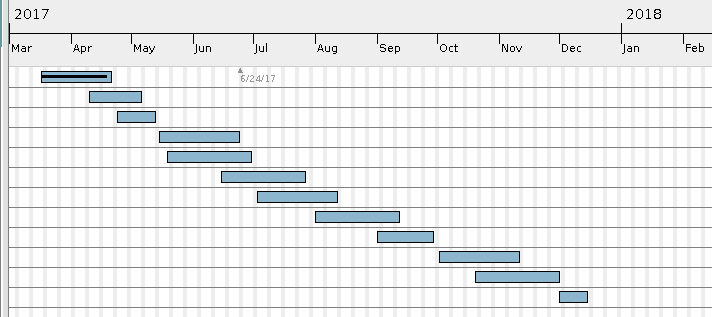
\includegraphics[scale=0.75]{figures/churngantt2.png}
% 	\caption{Gantt chart durations}
% 	\label{fig:time1}
% \end{figure}

%\newpage


%\end{landscape}

\FloatBarrier

%\setlength{\footskip}{8mm}

\chapter{Experimental Results}
\label{ch:results}

\textit{Some intro..}

\section{Section Name in Experimental Results}
\label{section-name-in-experimental-results}

Table~\ref{tab:hmm-based-detection-results} shows a table.

\begin{table}[t]
  \caption[Text shown in the LOT.]{\small Some table.}
  \begin{center}
    \begin{tabular}{c|c|c|c|c|c|c}
      \hline Batch method & TP & FP & TN & FN & TPR & FPR \\ \hline \hline
      Local ($z$-scoring) & 24 & 42 & 444 & 0 & 1 & 0.086 \\ \hline
      Local (LRT) & 24 & 486 & 0 & 0 & 1 & 1 \\ \hline 
      Global ($z$-scoring) & 24 & 217 & 10 & 0 & 1 & 0.956 \\ \hline 
      Global (LRT) & 24 & 223 & 4 & 0 & 1 & 0.982 \\ \hline
    \end{tabular}
  \end{center}
  \label{tab:hmm-based-detection-results}
\end{table} 

\FloatBarrier


\setlength{\footskip}{8mm}

\chapter{Conclusion and Recommendations}
\label{ch:conclusion}

This section presents the conclusion of study report.

\section{Conclusion}

In this paper we have tried to present a picture of the methods and tools of data analytics. They are summed up under three categories. Our motivation was to study the various methods and practices used by researchers and businesses.
We hope this paper encourage new companies to apply softwares and schemes to analyze data. The analytic results could give them insights about
To achieve what was not perceived, to deduce what was not understood is all made possible with data analytics. Thus it is our effort that the topics discussed in this paper would be of use to those who step into the world of Analytics without knowledge of background.

%\section{Recommendations}
%
%Text..

\FloatBarrier



% NEED TO CHANGE THE SECTION NUMBER FOR REFERENCES ACCORDINGLY.
\addcontentsline{toc}{chapter}{ \hskip 3.55em References}

\bibliographystyle{apacite}
\bibliography{references}


% COMMENT THE LINES ABOUT APPENDICS OUT IF YOU DO NOT HAVE THIS SECTION.

%%%%%%%%%%%%%%%%%%%%%%%%%%%%%%%%%%%%%%%%%%%%%%%%%%%%%%%%%%%%%%%%%%%
%                                                                 %
%                            APPENDICES                           %
%                                                                 %
%%%%%%%%%%%%%%%%%%%%%%%%%%%%%%%%%%%%%%%%%%%%%%%%%%%%%%%%%%%%%%%%%%%
\newpage\pagestyle{plain}
\theappendix

% NEED TO CHANGE THE SECTION NUMBER FOR REFERENCES ACCORDINGLY.
\addcontentsline{toc}{chapter}{7 \hskip 3.55em Appendices}

%\setlength{\footskip}{8mm}

% NOTE: NEED TO DO EVERYTHING SUCH AS SECTION NUMBER OR FIGURE NUMBER 
% MANUALLY IN THIS CHAPTER.

\renewcommand{\thefigure}{A.\arabic{figure}}

\begin{center}
{\large \bf Appendix A\\ \vskip 1em .. TITLE HERE ..\\ \vskip 1em}
\vskip 1em
\end{center}

\FloatBarrier

\singlespace
 
{\bf Section Name} \\ 

Figure~\ref{fig:monitoring-test} shows something. 

Some text ..

\begin{figure}[t]
  \centering
  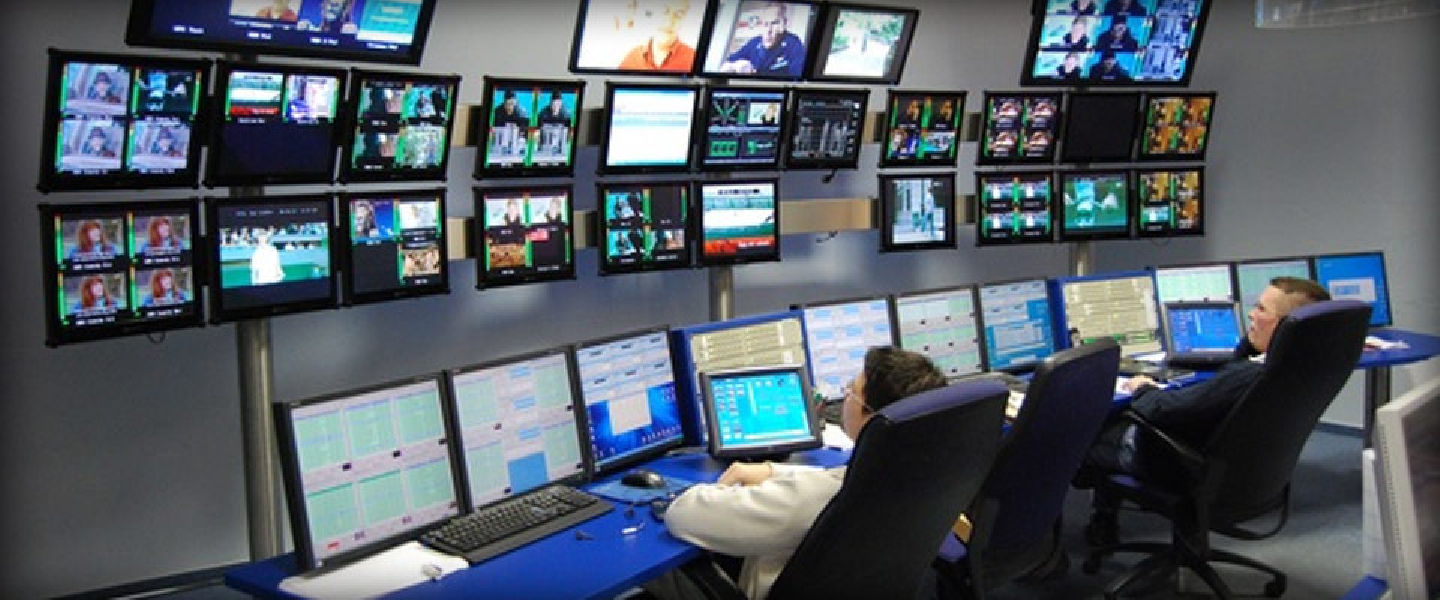
\includegraphics[width=5in]{figures/monitoring}
  \caption[CCTV monitoring room in Appendix A.]{\small CCTV monitoring
    room. Reprinted from the Twenty First Security Web site
    (\url{http://www.twentyfirstsecurity.com.au/}).}
  \label{fig:monitoring-test}
\end{figure}

\FloatBarrier



\end{document}
